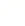
\includegraphics[width=0.34722in,height=0.36111in]{image1.png}

\textbf{初中数学}

\textbf{基础知识笔记}

目 录

第一篇、代数学\textbf{第一部分 有理实数}1.1.1 实数相关概念 11.1.2.
有理数运算 2\textbf{第二部分 无理实数}1.2.1. 根式 31.2.2.
\textbf{二次根式} 3\textbf{第三部分 整式与分式}1.3.1.
\textbf{整式概念与计算} 51.3.2. 因式分解 61.3.3. \textbf{分式概念与计算}
7第二篇、几何学\textbf{第一部分 相交线与平行线}2.1.1 相交线 92.1.2.
平行线 102.1.3. 命题与平移 10 \textbf{第二部分 三角形}2.2.1. 三角形性质
112.2.2. \textbf{特殊三角形} 122.2.3. \textbf{全等三角形} 132.2.4.
相似三角形 14\textbf{第三部分 四边形}2.3.1. \textbf{平行四边形} 152.3.2.
中点四边形 16\textbf{第四部分 圆}2.4.1. \textbf{圆有关概念} 172.4.2.
圆周角、圆心角定理 172.4.3. \textbf{直线与圆位置关系} 182.4.4. 圆幂定理
192.4.5. \textbf{扇形与圆锥} 19\textbf{第五部分 旋转与视图}2.5.1.
\textbf{旋转与对称} 202.5.2. 投影与视图 21\textbf{第六部分
几何解题方法与思路}2.6.1. 尺规作图 222.6.2 几何辅助线 222.6.3.
折叠、动点问题 242.6.4. 几何中的最值 242.6.5 圆考点梳理 262.6.6.
其它几何考点 27第三篇、方程、函数、不等式\textbf{第一部分 坐标系}3.1.1.
平面直角坐标系 29\textbf{第二部分 一次方程、函数与不等式}3.2.1.
\textbf{一元一次方程} 303.2.2. 二元一次方程组 313.2.3. \textbf{一次函数}
323.2.4. \textbf{一次不等式(组)} 333.2.5. 方程、函数、不等式关系
34\textbf{第三部分 分式方程与反比例函数}3.3.1. 分式方程 353.3.2.
反比例函数 36\textbf{第四部分 二次方程、函数与不等式}3.4.1.
\textbf{一元二次方程} 383.4.2. 二次函数 393.4.3.
\textbf{方程、函数、不等式关系} 40\textbf{第五部分 锐角三角函数}3.5.1.
锐角三角函数 42第四篇、统计概率\textbf{第一部分 统计}4.1.1.
\textbf{数据收集整理描述} 444.1.2. 统计分析 44\textbf{第二部分
概率}4.2.1. \textbf{事件和概率} 46

\hypertarget{ux4ee3ux6570ux5b66}{%
\section{\texorpdfstring{ 代数学}{ 代数学}}\label{ux4ee3ux6570ux5b66}}

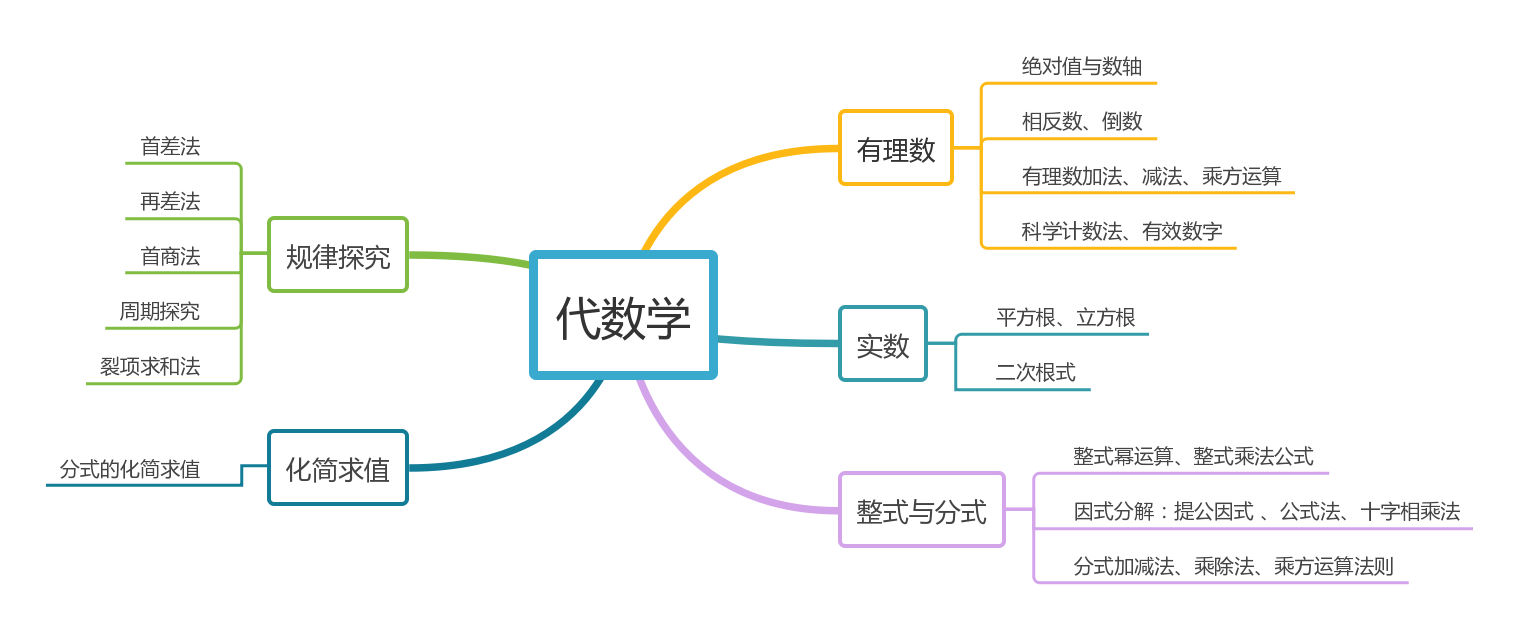
\includegraphics[width=6.97222in,height=2.61111in]{image4.png}

\hypertarget{ux6709ux7406ux5b9eux6570}{%
\subsection{\texorpdfstring{
有理实数}{ 有理实数}}\label{ux6709ux7406ux5b9eux6570}}

\hypertarget{ux5b66ux79d1ux7f51www.zxxk.com--ux6559ux80b2ux8d44ux6e90ux95e8ux6237ux63d0ux4f9bux8bd5ux9898ux8bd5ux5377ux6559ux6848ux8bfeux4ef6ux6559ux5b66ux8bbaux6587ux7d20ux6750ux7b49ux5404ux7c7bux6559ux5b66ux8d44ux6e90ux5e93ux4e0bux8f7dux8fd8ux6709ux5927ux91cfux4e30ux5bccux7684ux6559ux5b66ux8d44ux8baf}{%
\subsubsection{\texorpdfstring{\protect
\includegraphics[width=1.76389in,height=0.29167in]{image5.png}}{学科网(www.zxxk.com)-\/-教育资源门户,提供试题试卷、教案、课件、教学论文、素材等各类教学资源库下载,还有大量丰富的教学资讯!}}\label{ux5b66ux79d1ux7f51www.zxxk.com--ux6559ux80b2ux8d44ux6e90ux95e8ux6237ux63d0ux4f9bux8bd5ux9898ux8bd5ux5377ux6559ux6848ux8bfeux4ef6ux6559ux5b66ux8bbaux6587ux7d20ux6750ux7b49ux5404ux7c7bux6559ux5b66ux8d44ux6e90ux5e93ux4e0bux8f7dux8fd8ux6709ux5927ux91cfux4e30ux5bccux7684ux6559ux5b66ux8d44ux8baf}}

\textbf{1、有理数}

\textbf{(1)}定义:凡能写成为整数形式的数都是有理数。

\textbf{(2)}分类: ① ②

\textbf{2、实数分类}

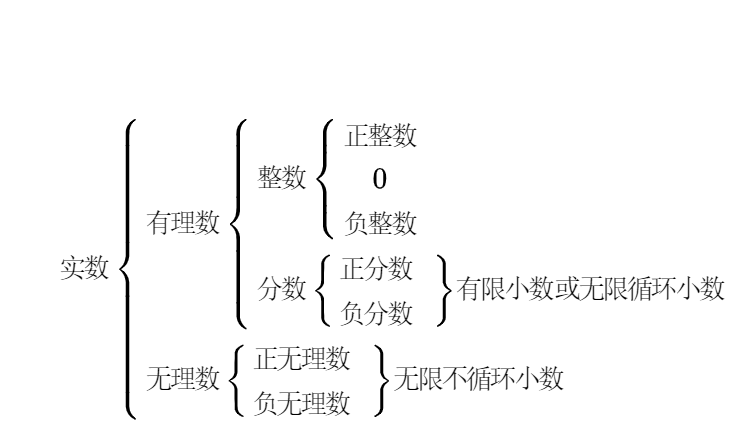
\includegraphics[width=3.40278in,height=1.55556in]{image6.png}

\textbf{★3、数轴:}数轴是规定了原点、正方向、单位长度的一条直线。

\includegraphics[width=2in,height=0.20833in]{image7.png}

①数轴三要素:原点、正方向、单位长度; ②实数和数轴上的点是一一对应的。

\textbf{★4、相反数:}符号不同的两个数,互为相反数;0的相反数还是0。其中:互为相反数。

\textbf{★5、绝对值}

\textbf{(1)}定义:数轴上表示某数的点离开原点的距离。

正数的绝对值是其本身,0的绝对值是0,负数的绝对值是它的相反数。

\textbf{(2)}绝对值可表示为: 或

\textbf{★6、倒数:}用1除以一个数的商,叫做这个数的倒数;乘积为1的两个数互为倒数,其中0没有倒数;

①若,那么的倒数是; ②实数互为倒数,则;

\hypertarget{ux5b66ux79d1ux7f51www.zxxk.com--ux6559ux80b2ux8d44ux6e90ux95e8ux6237ux63d0ux4f9bux8bd5ux9898ux8bd5ux5377ux6559ux6848ux8bfeux4ef6ux6559ux5b66ux8bbaux6587ux7d20ux6750ux7b49ux5404ux7c7bux6559ux5b66ux8d44ux6e90ux5e93ux4e0bux8f7dux8fd8ux6709ux5927ux91cfux4e30ux5bccux7684ux6559ux5b66ux8d44ux8baf-1}{%
\subsubsection{\texorpdfstring{\protect
\includegraphics[width=1.75in,height=0.34722in]{image5.png}}{学科网(www.zxxk.com)-\/-教育资源门户,提供试题试卷、教案、课件、教学论文、素材等各类教学资源库下载,还有大量丰富的教学资讯!}}\label{ux5b66ux79d1ux7f51www.zxxk.com--ux6559ux80b2ux8d44ux6e90ux95e8ux6237ux63d0ux4f9bux8bd5ux9898ux8bd5ux5377ux6559ux6848ux8bfeux4ef6ux6559ux5b66ux8bbaux6587ux7d20ux6750ux7b49ux5404ux7c7bux6559ux5b66ux8d44ux6e90ux5e93ux4e0bux8f7dux8fd8ux6709ux5927ux91cfux4e30ux5bccux7684ux6559ux5b66ux8d44ux8baf-1}}

\textbf{1、有理数运算法则}

\begin{longtable}[]{@{}lll@{}}
\toprule
\endhead
& 加法交换律: & 加法结合律:\tabularnewline
&
同号两数相加,取相同的符号并把绝对值相加;异号两数相加,取绝对值较大的符号,用较大的绝对值减去较小的绝对值
& 减去一个数,等于加上这个数的相反数,即。\tabularnewline
& 乘法交换律:、乘法结合律:、乘法分配律:. &\tabularnewline
\begin{minipage}[t]{0.30\columnwidth}\raggedright
\strut
\end{minipage} & \begin{minipage}[t]{0.30\columnwidth}\raggedright
两数相乘,同号为正,异号为负,并把绝对值相乘;几个数相乘,某因式为零,则积为零;各因式不为零,积的符号由负因式的个数决定.\strut
\end{minipage} & \begin{minipage}[t]{0.30\columnwidth}\raggedright
除以一个数等于乘以这个数的倒数;

注意:零不能做除数,.\strut
\end{minipage}\tabularnewline
\begin{minipage}[t]{0.30\columnwidth}\raggedright
\strut
\end{minipage} & \begin{minipage}[t]{0.30\columnwidth}\raggedright
求相同因式积的运算,叫做乘方;

乘方中,相同的因式叫做底数,相同因式的个数叫做指数,乘方的结果叫做幂;\strut
\end{minipage} & \begin{minipage}[t]{0.30\columnwidth}\raggedright
\strut
\end{minipage}\tabularnewline
&
⑴先算乘方,再算乘除,最后加减;⑵有括号先算括号;⑶同级运算,从左到右进行。
&\tabularnewline
\bottomrule
\end{longtable}

\textbf{★2、科学记数法:}把一个数或有限小数记成的形式,其中,为整数,这种记数法叫做科学记数法.

\begin{quote}
①原数的绝对值大于10时,利用科学记数法,写成的形式,注意,等于原数的整数位数减1,也是小数点向左移动的位数,如:.

②原数的绝对值小于10时,利用科学记数法,写成的形式,注意,等于原数左边第一个非0的数字前的所有0的个数,是小数点向右移动的位数,如:.
\end{quote}

\textbf{★3、近似数的精确:}一个近似数,四舍五入到那一位,就说这个近似数的精确到那一位.

\textbf{4、有效数字:}从左边第一个不为零的数字起,到精确的位数止,所有数字叫近似数的有效数字.

\hypertarget{ux65e0ux7406ux5b9eux6570}{%
\subsection{\texorpdfstring{
无理实数}{ 无理实数}}\label{ux65e0ux7406ux5b9eux6570}}


\includegraphics[width=1.75in,height=0.34722in]{image5.png}

\textbf{1、算术平方根:}如果一个非负数的平方等于,即,那么这个非负数叫做的算术平方根。

一个非负数的算术平方根记作读作根号或者读作二次根号。

\begin{longtable}[]{@{}l@{}}
\toprule
\endhead
\begin{minipage}[t]{0.97\columnwidth}\raggedright
★小结:算术平方根具有双重非负性:①负数没有算术平方根被开方数

②非负数的算术平方根只有一个且为正数的算术平方根等于本身\strut
\end{minipage}\tabularnewline
\bottomrule
\end{longtable}

\textbf{2、平方根:}如果一个数的平方等于,即,那么这个数叫做的平方根。

一个非负数的平方根记做读作正负根号或者读作正负二次根号。

\begin{longtable}[]{@{}l@{}}
\toprule
\endhead
\begin{minipage}[t]{0.97\columnwidth}\raggedright
★小结:正数的平方根有两个,互为相反数;0的平方根是0;负数没有平方根

开平方:求一个非负数的平方根的运算叫做开平方,非负数叫做被开方数。\strut
\end{minipage}\tabularnewline
\bottomrule
\end{longtable}

\textbf{3、立方根:}如果一个数的立方等于,即,那么这个数叫做的立方根三次方根。

一个数的立方根记做读作三次根号。

\begin{longtable}[]{@{}l@{}}
\toprule
\endhead
\begin{minipage}[t]{0.97\columnwidth}\raggedright
★小结:①任何一个数且只有一个立方根。

②正数的立方根为正数,负数的立方根为负数,0的立方根为0。\strut
\end{minipage}\tabularnewline
\bottomrule
\end{longtable}


\includegraphics[width=1.75in,height=0.34722in]{image5.png}

\textbf{1、二次根式的定义:}一般地,把形如的式子叫做二次根式。称为二次根号。

\textbf{★2、二次根式的性质:}

二次根式有意义的条件是,即只有被开方数时,式子才是二次根式,才有意义.

化简时,先将它化成,再根据绝对值的意义来进行化简.

中可以取任何实数,而中的必须取非负数;

\textbf{3、最简二次根式:}满足以下条件的根式叫最简二次根式

①被开方数不含分母(分母中也不能含有根号);
②被开方数不含能开得尽方的因数或因式。

\textbf{4、同类二次根式:}

化为最简二次根式后的被开方数相同,这样的二次根式叫做同类二次根式。

\textbf{★5、二次根式的运算}

\textbf{(1)}乘除法法则:算术平方根的积等于积的算术平方根:,

算术平方根的商等于商的算术平方根.,

\textbf{(2)}加减法法则:一般地,二次根式加减时,先将二次根式化成最简二次根式,再将被开方数相同的二次根式进行合并.二次根式进行加减运算时,实数的运算法则、运算律仍然适用.

\textbf{★6、分母有理化:}指将该原为无理数的分母化为有理数的过程,也就是将分母中的根号化去.

①单项式分母的分母有理化(运用有理化):

②分母中有一根号一数字或两个根号的分母有理化(运用平方差公式):

\textbf{7、实数大小的比较:}

(1)作差法:任意两个实数,若:

(2)作商法:任意两个实数,若:

(3)平方法:对含有根号的式子可以通过比较平方数的大小得根式大小。

\textbf{8、}绝对值、二次根式、平方三者都具有非负性,它们的任意搭配和为。

\hypertarget{ux6574ux5f0fux4e0eux5206ux5f0f}{%
\subsection{\texorpdfstring{
整式与分式}{ 整式与分式}}\label{ux6574ux5f0fux4e0eux5206ux5f0f}}

\hypertarget{ux5b66ux79d1ux7f51www.zxxk.com--ux6559ux80b2ux8d44ux6e90ux95e8ux6237ux63d0ux4f9bux8bd5ux9898ux8bd5ux5377ux6559ux6848ux8bfeux4ef6ux6559ux5b66ux8bbaux6587ux7d20ux6750ux7b49ux5404ux7c7bux6559ux5b66ux8d44ux6e90ux5e93ux4e0bux8f7dux8fd8ux6709ux5927ux91cfux4e30ux5bccux7684ux6559ux5b66ux8d44ux8baf-2}{%
\subsubsection{\texorpdfstring{\protect
\includegraphics[width=1.75in,height=0.34722in]{image5.png}}{学科网(www.zxxk.com)-\/-教育资源门户,提供试题试卷、教案、课件、教学论文、素材等各类教学资源库下载,还有大量丰富的教学资讯!}}\label{ux5b66ux79d1ux7f51www.zxxk.com--ux6559ux80b2ux8d44ux6e90ux95e8ux6237ux63d0ux4f9bux8bd5ux9898ux8bd5ux5377ux6559ux6848ux8bfeux4ef6ux6559ux5b66ux8bbaux6587ux7d20ux6750ux7b49ux5404ux7c7bux6559ux5b66ux8d44ux6e90ux5e93ux4e0bux8f7dux8fd8ux6709ux5927ux91cfux4e30ux5bccux7684ux6559ux5b66ux8d44ux8baf-2}}

\textbf{1、整式:}单项式和多项式统称为整式。

\textbf{(1)单项式:}数或字母的积组成的式子叫做单项式,单独的一个数或字母也是单项式。单项式中的数字因数叫做单项式的系数,一个单项式中所有字母的指数的和叫做单项式的次数。

\textbf{(2)多项式:}单项式的和叫做多项式。每个单项式叫多项式的项,不含字母的项叫做常数项,单项式的次数是几,就叫几次项。一个多项式中有几项,就叫~几项式。多项式里次数最高的项的次数,叫做多项式的次数。\\
\textbf{(3)同类项:}字母相同、字母的指数也相同叫同类项。同类项与系数、字母位置无关。合并是指同类项的系数相加作为新的系数,同类项的字母和字母的指数不变。

\textbf{2、整式的运算}

\textbf{(1)整式的加减法运算:}

\begin{quote}
①几个整式相加减,用括号把每个整式括起来,用加减号连接;然后去括号、合并同类项。\\
②化简求值的步骤:去括号合并同类项化到最简代入特殊值
\end{quote}

\textbf{★(2)指数幂运算}

①:同底数幂相乘,底数不变,指数相加。逆用公式:~

②:同底数幂相除,底数不变,指数相减。逆用公式:

③:幂的乘方,底数不变,指数相乘。逆用公式:

④:积的乘方,等于积的因式乘方积。~逆用公式:

⑤任何不等于0的数的0次幂都等于1。即

⑥负整数指数幂:

\textbf{(3)整式乘除法运算:}

\begin{quote}
\textbf{①单项式的乘除法法则:}单项式与单项式相乘,把它们的系数,相同字母分别相乘,对于只在一个单项式里含有的字母,则连同它们的指数作为积的一个因式;单项式相除,把系数与同底数幂分别相除作为商的因式,对于只有被除式里含有的字母,则连同它的指数作为商的一个因式.

\textbf{②单项式与多项式相乘的法则:}
~单项式与多项式相乘,就是用单项式去乘多项式的每一项,再把所得的积相加.即

\textbf{③多项式与多项式乘法法则:}多项式与多项式相乘,先用一个多项式的每一项乘另一个多项式的每一项,再把所得的积相加.即.
\end{quote}

\textbf{★(4)整式乘法公式 ~}

平方差公式: ~

完全平方公式:

以下是常见的变形: ~

\hypertarget{ux5b66ux79d1ux7f51www.zxxk.com--ux6559ux80b2ux8d44ux6e90ux95e8ux6237ux63d0ux4f9bux8bd5ux9898ux8bd5ux5377ux6559ux6848ux8bfeux4ef6ux6559ux5b66ux8bbaux6587ux7d20ux6750ux7b49ux5404ux7c7bux6559ux5b66ux8d44ux6e90ux5e93ux4e0bux8f7dux8fd8ux6709ux5927ux91cfux4e30ux5bccux7684ux6559ux5b66ux8d44ux8baf-3}{%
\subsubsection{\texorpdfstring{\protect
\includegraphics[width=1.75in,height=0.34722in]{image5.png}}{学科网(www.zxxk.com)-\/-教育资源门户,提供试题试卷、教案、课件、教学论文、素材等各类教学资源库下载,还有大量丰富的教学资讯!}}\label{ux5b66ux79d1ux7f51www.zxxk.com--ux6559ux80b2ux8d44ux6e90ux95e8ux6237ux63d0ux4f9bux8bd5ux9898ux8bd5ux5377ux6559ux6848ux8bfeux4ef6ux6559ux5b66ux8bbaux6587ux7d20ux6750ux7b49ux5404ux7c7bux6559ux5b66ux8d44ux6e90ux5e93ux4e0bux8f7dux8fd8ux6709ux5927ux91cfux4e30ux5bccux7684ux6559ux5b66ux8d44ux8baf-3}}

\textbf{1、概念:}把一个多项式化成几个整式积的形式,叫做因式分解,也叫分解因式。

\textbf{★2、因式分解的方法:}

\textbf{(1)提公因式法:}多项式的各项中都含有相同的因式,那么这个相同的因式就叫做公因式。把多项式分解成两个因式的乘积的形式,即。

①用提公因式法分解因式的关键是准确找出多项式各项的公因式.如:

\begin{quote}
②当多项式第一项的系数是负数时,先提出``---''号,使括号内的第一项的系数变为正数,同时多项式的各项都要变号.如:

③用提公因式法分解因式时,若多项式的某项与公因式相等或它们的和为零,则提取公因式后,该项变为:``+''或``-'',不要把该项漏掉,或认为是而出现错误。
\end{quote}

如:

\textbf{★(2)公式法:}利用平方差公式:和完全平方公式:对多项式进行因式分解的方法。如:

\begin{quote}
对多项式可以先用整体法,即先令,则上式变为,简单明了,继续用公式法分解因式。
\end{quote}

\textbf{★(3)十字相乘法
:}利用十字交叉线来分解系数,把\textbf{二次三项式}分解因式的方法叫做十字相乘法。

对于二次三项式,若存在 ,则

判断方法:拆\textbf{二次项}与\textbf{常数项,}交叉相乘\textbf{和为一次项}即可用该方法。判断时十字交叉,书写时横向相加再相乘。在二次三项式(≠0)中,如果二次项系数可以分解成两个因数之积,即,常数项可以分解成两个因数之积,即,把排列如下:

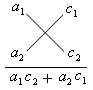
\includegraphics[width=0.97222in,height=0.94444in]{image8.png}

按斜线交叉相乘,再相加,得到,若它正好等于二次三项式的一次项系数,即,则二次三项式可分解为两因式与之积,即.

\textbf{举例:}

\hypertarget{ux5b66ux79d1ux7f51www.zxxk.com--ux6559ux80b2ux8d44ux6e90ux95e8ux6237ux63d0ux4f9bux8bd5ux9898ux8bd5ux5377ux6559ux6848ux8bfeux4ef6ux6559ux5b66ux8bbaux6587ux7d20ux6750ux7b49ux5404ux7c7bux6559ux5b66ux8d44ux6e90ux5e93ux4e0bux8f7dux8fd8ux6709ux5927ux91cfux4e30ux5bccux7684ux6559ux5b66ux8d44ux8baf-4}{%
\subsubsection{\texorpdfstring{\protect
\includegraphics[width=1.75in,height=0.34722in]{image5.png}}{学科网(www.zxxk.com)-\/-教育资源门户,提供试题试卷、教案、课件、教学论文、素材等各类教学资源库下载,还有大量丰富的教学资讯!}}\label{ux5b66ux79d1ux7f51www.zxxk.com--ux6559ux80b2ux8d44ux6e90ux95e8ux6237ux63d0ux4f9bux8bd5ux9898ux8bd5ux5377ux6559ux6848ux8bfeux4ef6ux6559ux5b66ux8bbaux6587ux7d20ux6750ux7b49ux5404ux7c7bux6559ux5b66ux8d44ux6e90ux5e93ux4e0bux8f7dux8fd8ux6709ux5927ux91cfux4e30ux5bccux7684ux6559ux5b66ux8d44ux8baf-4}}

\textbf{1、分式定义:}如果表示两个整数,并且中含有字母,那么式子叫做分式。

\textbf{★2、与分式有关的条件}

①分式有意义:分母不为 分式无意义:分母为

②分式值为:分子为且分母不为,

\textbf{★3、分式的性质}

\begin{quote}
①基本性质:,为不等于的整式.\\
②最简分式:分子与分母没有公因式的分式叫做最简分式.如果分子分母有公因式,要进行约分化简.
\end{quote}

\textbf{3、分式的运算}

\textbf{(1)分式的加减:}同分母分式相加减,分母不变,把分子相加减,

异分母分式相加减,先通分,变为同分母的分式,再加减,.

★关于通分:单项式分母以数字最小公倍数和字母最高次项的积为公分母。

多项式先进行因式分解,然后以公因式和各项的独因式积为公分母。

整式与分式相加减时,对整式进行通分,以分式的分母为分母,整式乘分母为分子。

\textbf{(2)分式的乘除法法则:}

分式乘分式,用分子的积作为积的分子,分母的积作为积的分母,

分式除以分式,把除式的分子、分母颠倒位置后,与被除式相乘,

★①分式与分式相乘,若分子和分母是多项式,则先分解因式,看能否约分,然后再乘。

②整式与分式相乘,可以直接把整式(整式可以看作分母是的代数式)和分式的分子相乘作为分子,分母不变.当整式是多项式时,同样要先分解因式,便于约分。

\textbf{(3)分式的乘方法则:}分式的乘方是把分子、分母分别乘方,用字母表示为:

★分式乘方时,应把分子、分母分别看作一个整体.如.

\hypertarget{ux51e0ux4f55ux5b66}{%
\section{\texorpdfstring{ 几何学}{ 几何学}}\label{ux51e0ux4f55ux5b66}}

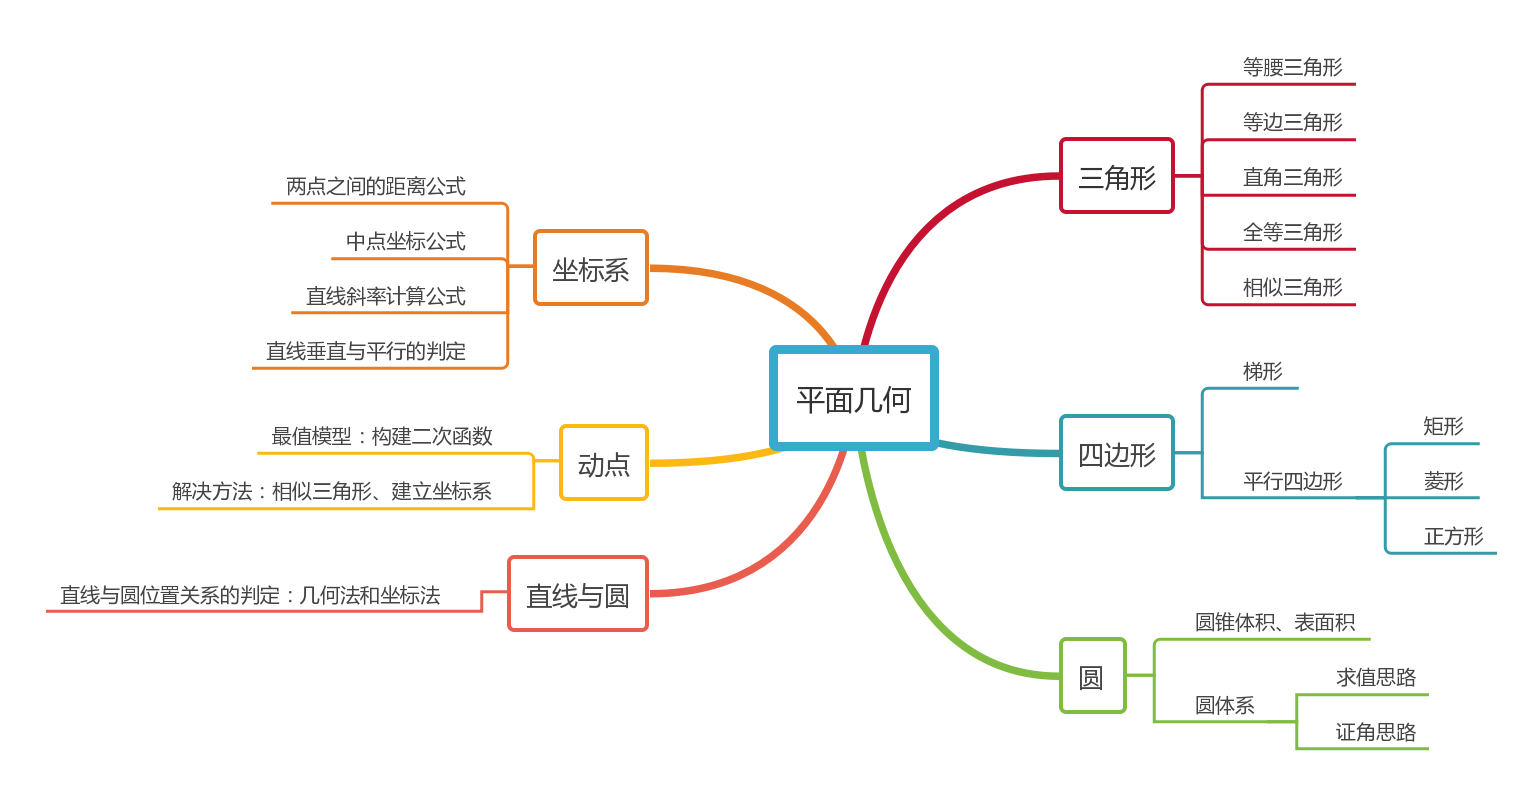
\includegraphics[width=6.47222in,height=3.16667in]{image9.png}

\hypertarget{ux76f8ux4ea4ux7ebfux4e0eux5e73ux884cux7ebf}{%
\subsection{\texorpdfstring{
相交线与平行线}{ 相交线与平行线}}\label{ux76f8ux4ea4ux7ebfux4e0eux5e73ux884cux7ebf}}

\hypertarget{ux5b66ux79d1ux7f51www.zxxk.com--ux6559ux80b2ux8d44ux6e90ux95e8ux6237ux63d0ux4f9bux8bd5ux9898ux8bd5ux5377ux6559ux6848ux8bfeux4ef6ux6559ux5b66ux8bbaux6587ux7d20ux6750ux7b49ux5404ux7c7bux6559ux5b66ux8d44ux6e90ux5e93ux4e0bux8f7dux8fd8ux6709ux5927ux91cfux4e30ux5bccux7684ux6559ux5b66ux8d44ux8baf-5}{%
\subsubsection{\texorpdfstring{\protect
\includegraphics[width=1.75in,height=0.34722in]{image5.png}}{学科网(www.zxxk.com)-\/-教育资源门户,提供试题试卷、教案、课件、教学论文、素材等各类教学资源库下载,还有大量丰富的教学资讯!}}\label{ux5b66ux79d1ux7f51www.zxxk.com--ux6559ux80b2ux8d44ux6e90ux95e8ux6237ux63d0ux4f9bux8bd5ux9898ux8bd5ux5377ux6559ux6848ux8bfeux4ef6ux6559ux5b66ux8bbaux6587ux7d20ux6750ux7b49ux5404ux7c7bux6559ux5b66ux8d44ux6e90ux5e93ux4e0bux8f7dux8fd8ux6709ux5927ux91cfux4e30ux5bccux7684ux6559ux5b66ux8d44ux8baf-5}}

\textbf{1、对顶角与邻补角}

\begin{longtable}[]{@{}lllll@{}}
\toprule
\endhead
& & & &\tabularnewline
\begin{minipage}[t]{0.17\columnwidth}\raggedright
\strut
\end{minipage} & \begin{minipage}[t]{0.17\columnwidth}\raggedright
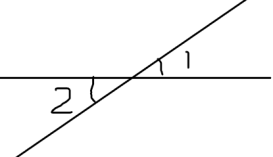
\includegraphics[width=1.23611in,height=0.70833in]{image10.png}\strut
\end{minipage} & \begin{minipage}[t]{0.17\columnwidth}\raggedright
有公共顶点\strut
\end{minipage} & \begin{minipage}[t]{0.17\columnwidth}\raggedright
的两边与

的两边互为反向延长线\strut
\end{minipage} & \begin{minipage}[t]{0.17\columnwidth}\raggedright
对顶角相等

即\strut
\end{minipage}\tabularnewline
&
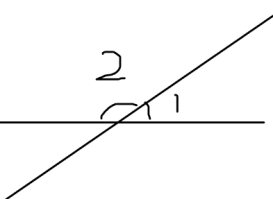
\includegraphics[width=1.23611in,height=0.90278in]{image11.png}
& 有公共顶点 & 与有一条边公共,另一边互为反向延长线. &
邻补角互补即\tabularnewline
\bottomrule
\end{longtable}

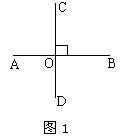
\includegraphics[width=1.31944in,height=1.15278in]{image12.png}

\textbf{2、垂线}

\textbf{①定义:}当两条直线相交所成的四个角中,有一个角是直角时,就说这两条直线互相垂直,
其中的一条直线叫做另一条直线的垂线,它们的交点叫做垂足.如图所示,符号语言记作:
,垂足为。

\textbf{②垂线的性质:}

垂线性质:在同一平面内,过一点有且只有一条直线与已知直线垂直
(与平行公理相比较记)。

垂线性质:连接直线外一点与直线上各点的所有线段中,垂线段最短.简称:垂线段最短。

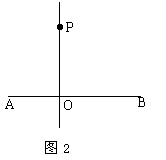
\includegraphics[width=1.58333in,height=1.20833in]{image13.png}

\textbf{③点到直线的距离:}直线外一点到这条直线的垂线段的长度,叫做点到直线的距离。如图,,点到直线的距离是垂线段的长.

\hypertarget{ux5b66ux79d1ux7f51www.zxxk.com--ux6559ux80b2ux8d44ux6e90ux95e8ux6237ux63d0ux4f9bux8bd5ux9898ux8bd5ux5377ux6559ux6848ux8bfeux4ef6ux6559ux5b66ux8bbaux6587ux7d20ux6750ux7b49ux5404ux7c7bux6559ux5b66ux8d44ux6e90ux5e93ux4e0bux8f7dux8fd8ux6709ux5927ux91cfux4e30ux5bccux7684ux6559ux5b66ux8d44ux8baf-6}{%
\subsubsection{\texorpdfstring{\protect
\includegraphics[width=1.75in,height=0.34722in]{image5.png}}{学科网(www.zxxk.com)-\/-教育资源门户,提供试题试卷、教案、课件、教学论文、素材等各类教学资源库下载,还有大量丰富的教学资讯!}}\label{ux5b66ux79d1ux7f51www.zxxk.com--ux6559ux80b2ux8d44ux6e90ux95e8ux6237ux63d0ux4f9bux8bd5ux9898ux8bd5ux5377ux6559ux6848ux8bfeux4ef6ux6559ux5b66ux8bbaux6587ux7d20ux6750ux7b49ux5404ux7c7bux6559ux5b66ux8d44ux6e90ux5e93ux4e0bux8f7dux8fd8ux6709ux5927ux91cfux4e30ux5bccux7684ux6559ux5b66ux8d44ux8baf-6}}

\textbf{★1、性质与判定}

\textbf{①性质:}两直线平行同位角相等、内错角相等、同旁内角互补

\textbf{②判定:}同位角相等、内错角相等、同旁内角互补两直线平行

\textbf{2、平行线的构造}

\begin{longtable}[]{@{}llllll@{}}
\toprule
\endhead
& & & & &\tabularnewline
&
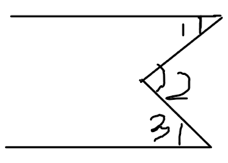
\includegraphics[width=1.03542in,height=0.73889in]{image14.png}
&
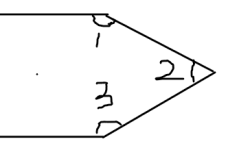
\includegraphics[width=1.03611in,height=0.68333in]{image15.png}
&
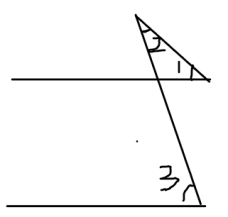
\includegraphics[width=1.03681in,height=0.98819in]{image16.png}
&
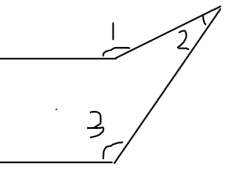
\includegraphics[width=1.03611in,height=0.78542in]{image17.png}
&
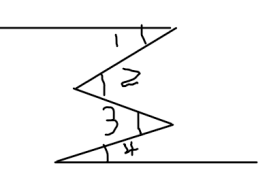
\includegraphics[width=1.2125in,height=0.84097in]{image18.png}\tabularnewline
& & & & &\tabularnewline
\bottomrule
\end{longtable}

\hypertarget{ux5b66ux79d1ux7f51www.zxxk.com--ux6559ux80b2ux8d44ux6e90ux95e8ux6237ux63d0ux4f9bux8bd5ux9898ux8bd5ux5377ux6559ux6848ux8bfeux4ef6ux6559ux5b66ux8bbaux6587ux7d20ux6750ux7b49ux5404ux7c7bux6559ux5b66ux8d44ux6e90ux5e93ux4e0bux8f7dux8fd8ux6709ux5927ux91cfux4e30ux5bccux7684ux6559ux5b66ux8d44ux8baf-7}{%
\subsubsection{\texorpdfstring{\protect
\includegraphics[width=1.75in,height=0.34722in]{image5.png}}{学科网(www.zxxk.com)-\/-教育资源门户,提供试题试卷、教案、课件、教学论文、素材等各类教学资源库下载,还有大量丰富的教学资讯!}}\label{ux5b66ux79d1ux7f51www.zxxk.com--ux6559ux80b2ux8d44ux6e90ux95e8ux6237ux63d0ux4f9bux8bd5ux9898ux8bd5ux5377ux6559ux6848ux8bfeux4ef6ux6559ux5b66ux8bbaux6587ux7d20ux6750ux7b49ux5404ux7c7bux6559ux5b66ux8d44ux6e90ux5e93ux4e0bux8f7dux8fd8ux6709ux5927ux91cfux4e30ux5bccux7684ux6559ux5b66ux8d44ux8baf-7}}

\textbf{1、命题:}判断一件事情的语句,叫做命题.每个命题都是题设、结论两部分组成.题设是已知事项;结论是由已知事项推出的事项。

\textbf{2、常见结论及其否定形式}

\begin{longtable}[]{@{}llll@{}}
\toprule
\endhead
& & &\tabularnewline
\textbf{是} & \textbf{不是} & \textbf{至少有一个} &
\textbf{一个也没有}\tabularnewline
\textbf{都是} & \textbf{不都是} & \textbf{至多有一个} &
\textbf{至少有两个}\tabularnewline
\textbf{大于} & \textbf{不大于(小于等于)} & \textbf{至少有个} &
\textbf{至多有()个}\tabularnewline
\textbf{小于} & \textbf{不小于(大于等于)} & \textbf{至多有个} &
\textbf{至少有()个}\tabularnewline
\textbf{对所有,成立} & \textbf{存在某,不成立} & \textbf{或} &
\textbf{且}\tabularnewline
\textbf{对任何,不成立} & \textbf{存在某,成立} & \textbf{且} &
\textbf{或}\tabularnewline
\bottomrule
\end{longtable}

\textbf{3、平移:}在平面内,将一个图形沿某个方向移动一定的距离,图形的这种移动叫做平移。

\textbf{平移的性质:}平移后,对应线段平行(或共线)且相等,对应角相等,对应点所连线段平行(或共线)且相等

\hypertarget{ux4e09ux89d2ux5f62}{%
\subsection{\texorpdfstring{
三角形}{ 三角形}}\label{ux4e09ux89d2ux5f62}}

\hypertarget{ux5b66ux79d1ux7f51www.zxxk.com--ux6559ux80b2ux8d44ux6e90ux95e8ux6237ux63d0ux4f9bux8bd5ux9898ux8bd5ux5377ux6559ux6848ux8bfeux4ef6ux6559ux5b66ux8bbaux6587ux7d20ux6750ux7b49ux5404ux7c7bux6559ux5b66ux8d44ux6e90ux5e93ux4e0bux8f7dux8fd8ux6709ux5927ux91cfux4e30ux5bccux7684ux6559ux5b66ux8d44ux8baf-8}{%
\subsubsection{\texorpdfstring{\protect
\includegraphics[width=1.75in,height=0.34722in]{image5.png}}{学科网(www.zxxk.com)-\/-教育资源门户,提供试题试卷、教案、课件、教学论文、素材等各类教学资源库下载,还有大量丰富的教学资讯!}}\label{ux5b66ux79d1ux7f51www.zxxk.com--ux6559ux80b2ux8d44ux6e90ux95e8ux6237ux63d0ux4f9bux8bd5ux9898ux8bd5ux5377ux6559ux6848ux8bfeux4ef6ux6559ux5b66ux8bbaux6587ux7d20ux6750ux7b49ux5404ux7c7bux6559ux5b66ux8d44ux6e90ux5e93ux4e0bux8f7dux8fd8ux6709ux5927ux91cfux4e30ux5bccux7684ux6559ux5b66ux8d44ux8baf-8}}

\textbf{★1、构成三角形的条件:}两边之和大于第三边或两边之和小于第三边

\textbf{★2、三角形内角和定理:}三角形的内角和为

\textbf{推论}:三角形的外角等于与它不相邻的两内角和。

\textbf{3、分类}

①按角分类: ②按边分类:

\textbf{★4、多边形}

①多边形内角和。若正多边形每个内角为,则有

②多边形外角和。若正多边形每个外角为,则有

③多边形对角线条数

\textbf{★5、三角形中的线段}

\begin{longtable}[]{@{}lllll@{}}
\toprule
\endhead
& & & &\tabularnewline
&
从三角形的一顶点向它的对边作垂线,顶点和垂足之间的线段叫做三角形的高线。
&
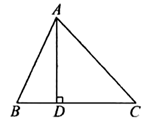
\includegraphics[width=1.16667in,height=0.95833in]{image19.png}
& 在底边上的高为。 &\tabularnewline
& 三角形的一顶点与它的对边中点的连线叫三角形的中线. &
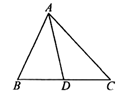
\includegraphics[width=1.13889in,height=0.88889in]{image20.png}
& 在底边上的中线为。 &\tabularnewline
\begin{minipage}[t]{0.17\columnwidth}\raggedright
\strut
\end{minipage} & \begin{minipage}[t]{0.17\columnwidth}\raggedright
三角形一个内角的平分线与它的对边相交,这个角的顶点与交点之间的线段叫做三角形的角平分线.\strut
\end{minipage} & \begin{minipage}[t]{0.17\columnwidth}\raggedright
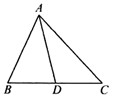
\includegraphics[width=1.05556in,height=0.90278in]{image21.png}\strut
\end{minipage} & \begin{minipage}[t]{0.17\columnwidth}\raggedright
在顶角

上的角平

分线为。\strut
\end{minipage} & \begin{minipage}[t]{0.17\columnwidth}\raggedright
\strut
\end{minipage}\tabularnewline
& 三角形两边中点的连线叫中位线。 &
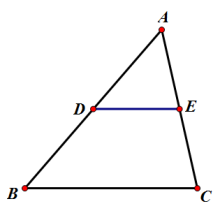
\includegraphics[width=1.20833in,height=1.16667in]{image22.png}
& 三角形的中位线平行于第三边,并且等于第三边的一半。 &\tabularnewline
\bottomrule
\end{longtable}

\textbf{5、三角形的三心}

\textbf{(1)重心:}三角形三条中线的交点叫三角形的重心。

重心性质:重心和三角形顶点组成的个三角形面积相等

重心到顶点的距离与重心到底边中点距离之比为

三角形顶点坐标则重心坐标为

\textbf{(2)内心:}三角形三内角角平分线交点叫三角形内心,是三角形内切圆圆心。

内心性质:内心到三角形三边的距离相等

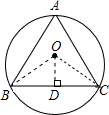
\includegraphics[width=0.875in,height=0.93056in]{image24.png}

三角形面积与内切圆半径关系:

\textbf{(3)外心:}三角形三边垂直平分线的交点叫三角形外心,是三角形外接圆圆心。

外心性质:外心到三角形三顶点的距离相等;三角形面积与外接圆半径关系:

\hypertarget{ux5b66ux79d1ux7f51www.zxxk.com--ux6559ux80b2ux8d44ux6e90ux95e8ux6237ux63d0ux4f9bux8bd5ux9898ux8bd5ux5377ux6559ux6848ux8bfeux4ef6ux6559ux5b66ux8bbaux6587ux7d20ux6750ux7b49ux5404ux7c7bux6559ux5b66ux8d44ux6e90ux5e93ux4e0bux8f7dux8fd8ux6709ux5927ux91cfux4e30ux5bccux7684ux6559ux5b66ux8d44ux8baf-9}{%
\subsubsection{\texorpdfstring{\protect
\includegraphics[width=1.75in,height=0.34722in]{image5.png}}{学科网(www.zxxk.com)-\/-教育资源门户,提供试题试卷、教案、课件、教学论文、素材等各类教学资源库下载,还有大量丰富的教学资讯!}}\label{ux5b66ux79d1ux7f51www.zxxk.com--ux6559ux80b2ux8d44ux6e90ux95e8ux6237ux63d0ux4f9bux8bd5ux9898ux8bd5ux5377ux6559ux6848ux8bfeux4ef6ux6559ux5b66ux8bbaux6587ux7d20ux6750ux7b49ux5404ux7c7bux6559ux5b66ux8d44ux6e90ux5e93ux4e0bux8f7dux8fd8ux6709ux5927ux91cfux4e30ux5bccux7684ux6559ux5b66ux8d44ux8baf-9}}

\begin{longtable}[]{@{}llll@{}}
\toprule
\endhead
& & &\tabularnewline
& 定义 &
有两条边相等的三角形,叫等腰三角形。相等的两边叫腰,另一条边叫做底边,两腰所夹的角叫顶角,底边与腰的夹角叫做底角
&
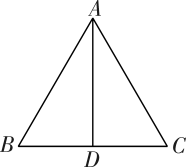
\includegraphics[width=1.25in,height=1.125in]{image25.png}\tabularnewline
\begin{minipage}[t]{0.22\columnwidth}\raggedright
\strut
\end{minipage} & \begin{minipage}[t]{0.22\columnwidth}\raggedright
性质\strut
\end{minipage} & \begin{minipage}[t]{0.22\columnwidth}\raggedright
①等腰三角形是轴对称图形

②等腰三角形的两个底角相等(等边对等角)

③等腰三角形的顶角平分线、底边中线、高线相互重合(三线合一)\strut
\end{minipage} & \begin{minipage}[t]{0.22\columnwidth}\raggedright
\strut
\end{minipage}\tabularnewline
\begin{minipage}[t]{0.22\columnwidth}\raggedright
\strut
\end{minipage} & \begin{minipage}[t]{0.22\columnwidth}\raggedright
判定\strut
\end{minipage} & \begin{minipage}[t]{0.22\columnwidth}\raggedright
①两边相等、两底角相等为等腰三角形。

②两线合一两三角形全等为等腰三角形。\strut
\end{minipage} & \begin{minipage}[t]{0.22\columnwidth}\raggedright
\strut
\end{minipage}\tabularnewline
& 定义 &
三条边都相等的三角形是等边三角形,等边三角形是特殊的等腰三角形。 &
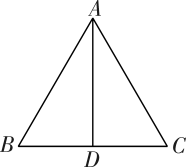
\includegraphics[width=1.25in,height=1.125in]{image25.png}\tabularnewline
& 性质 & 等边三角形的三边都相等,三个内角都相等,并且每一个角都等于60°。
&\tabularnewline
\begin{minipage}[t]{0.22\columnwidth}\raggedright
\strut
\end{minipage} & \begin{minipage}[t]{0.22\columnwidth}\raggedright
判定\strut
\end{minipage} & \begin{minipage}[t]{0.22\columnwidth}\raggedright
①三边都相等的三角形是等边三角形。

②三个角都相等的三角形是等边三角形。

③有两个角是60°的三角形是等边三角形。

④有一个角是60°的等腰三角形是等边三角形。\strut
\end{minipage} & \begin{minipage}[t]{0.22\columnwidth}\raggedright
\strut
\end{minipage}\tabularnewline
& 定义 & 有一个角是直角的三角形叫做直角三角形。 &
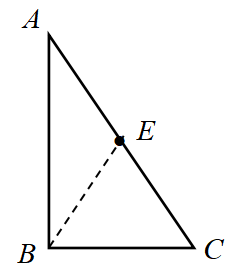
\includegraphics[width=1.25in,height=1.48611in]{image26.png}\tabularnewline
\begin{minipage}[t]{0.22\columnwidth}\raggedright
\strut
\end{minipage} & \begin{minipage}[t]{0.22\columnwidth}\raggedright
性质\strut
\end{minipage} & \begin{minipage}[t]{0.22\columnwidth}\raggedright
①直角三角形的两锐角互余。

②在直角三角形中,如果一个锐角等于°,那么它所对的直角边等于斜边的一半。

③在直角三角形中,斜边上的中线等于斜边的一半。

④勾股定理:在任何一个直角三角形中,两条直角边长的平方之和一定等于斜边长的平方,即。\strut
\end{minipage} & \begin{minipage}[t]{0.22\columnwidth}\raggedright
\strut
\end{minipage}\tabularnewline
\begin{minipage}[t]{0.22\columnwidth}\raggedright
\strut
\end{minipage} & \begin{minipage}[t]{0.22\columnwidth}\raggedright
判定\strut
\end{minipage} & \begin{minipage}[t]{0.22\columnwidth}\raggedright
①含有°角(两锐角互余)的三角形是直角三角形。

②勾股定理的逆定理:如果三角形的三条边存在关系``\,'',那么这个三角形是直角三角形。

③如果三角形一边上的中线等于这条边的一半,那么这个三角形是直角三角形。\strut
\end{minipage} & \begin{minipage}[t]{0.22\columnwidth}\raggedright
\strut
\end{minipage}\tabularnewline
& 实记勾股数 &
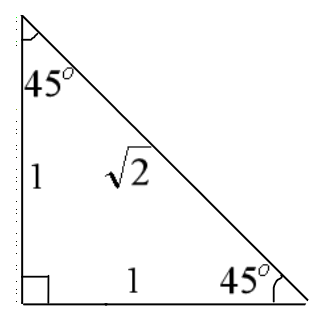
\includegraphics[width=1.13889in,height=1.19444in]{image27.png}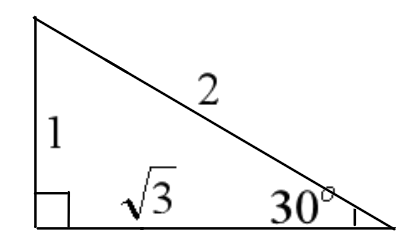
\includegraphics[width=1.68056in,height=0.98611in]{image28.png}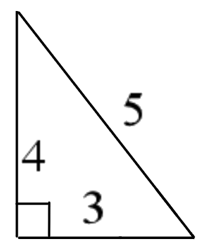
\includegraphics[width=0.875in,height=1.08333in]{image29.png}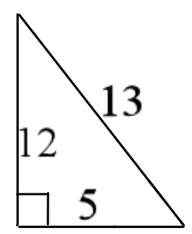
\includegraphics[width=0.81944in,height=1.01389in]{image30.png}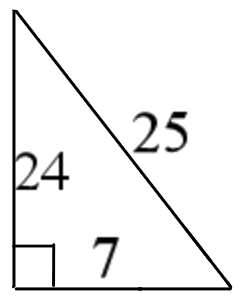
\includegraphics[width=0.90278in,height=1.16667in]{image31.png}
&\tabularnewline
\bottomrule
\end{longtable}

\hypertarget{section}{%
\subsubsection{}\label{section}}

\hypertarget{ux5b66ux79d1ux7f51www.zxxk.com--ux6559ux80b2ux8d44ux6e90ux95e8ux6237ux63d0ux4f9bux8bd5ux9898ux8bd5ux5377ux6559ux6848ux8bfeux4ef6ux6559ux5b66ux8bbaux6587ux7d20ux6750ux7b49ux5404ux7c7bux6559ux5b66ux8d44ux6e90ux5e93ux4e0bux8f7dux8fd8ux6709ux5927ux91cfux4e30ux5bccux7684ux6559ux5b66ux8d44ux8baf-10}{%
\subsubsection{\texorpdfstring{\protect
\includegraphics[width=1.75in,height=0.34722in]{image5.png}}{学科网(www.zxxk.com)-\/-教育资源门户,提供试题试卷、教案、课件、教学论文、素材等各类教学资源库下载,还有大量丰富的教学资讯!}}\label{ux5b66ux79d1ux7f51www.zxxk.com--ux6559ux80b2ux8d44ux6e90ux95e8ux6237ux63d0ux4f9bux8bd5ux9898ux8bd5ux5377ux6559ux6848ux8bfeux4ef6ux6559ux5b66ux8bbaux6587ux7d20ux6750ux7b49ux5404ux7c7bux6559ux5b66ux8d44ux6e90ux5e93ux4e0bux8f7dux8fd8ux6709ux5927ux91cfux4e30ux5bccux7684ux6559ux5b66ux8d44ux8baf-10}}

\begin{longtable}[]{@{}lll@{}}
\toprule
\endhead
& &\tabularnewline
& 两三角形全等对应角相等、对应边相等。 &
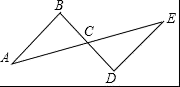
\includegraphics[width=1.44444in,height=0.69444in]{image32.png}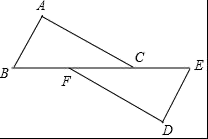
\includegraphics[width=1.43056in,height=0.95833in]{image33.png}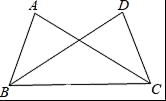
\includegraphics[width=1.30556in,height=0.79167in]{image34.png}\tabularnewline
\begin{minipage}[t]{0.30\columnwidth}\raggedright
\strut
\end{minipage} & \begin{minipage}[t]{0.30\columnwidth}\raggedright
①边边边:三边分别相等的两个三角形全等

②边角边:两边分别相等且夹角也相等的两个三角形全等

③角边角:两角对应相等且夹边也相等的两个三角形全等

④角角边:两角对应相等且有一边也相等的两个三角形全等

⑤:直角三角形中对应直角边和斜边分别相等的两个三角形全等\strut
\end{minipage} & \begin{minipage}[t]{0.30\columnwidth}\raggedright
\strut
\end{minipage}\tabularnewline
\begin{minipage}[t]{0.30\columnwidth}\raggedright
\strut
\end{minipage} & \begin{minipage}[t]{0.30\columnwidth}\raggedright
\hypertarget{ux5728ux4e0eux4e2d}{%
\subsubsection{在与中 ∵ ∴≌}\label{ux5728ux4e0eux4e2d}}\strut
\end{minipage} & \begin{minipage}[t]{0.30\columnwidth}\raggedright
\strut
\end{minipage}\tabularnewline
\bottomrule
\end{longtable}

\hypertarget{ux5b66ux79d1ux7f51www.zxxk.com--ux6559ux80b2ux8d44ux6e90ux95e8ux6237ux63d0ux4f9bux8bd5ux9898ux8bd5ux5377ux6559ux6848ux8bfeux4ef6ux6559ux5b66ux8bbaux6587ux7d20ux6750ux7b49ux5404ux7c7bux6559ux5b66ux8d44ux6e90ux5e93ux4e0bux8f7dux8fd8ux6709ux5927ux91cfux4e30ux5bccux7684ux6559ux5b66ux8d44ux8baf-11}{%
\subsubsection{\texorpdfstring{\protect
\includegraphics[width=1.75in,height=0.34722in]{image5.png}}{学科网(www.zxxk.com)-\/-教育资源门户,提供试题试卷、教案、课件、教学论文、素材等各类教学资源库下载,还有大量丰富的教学资讯!}}\label{ux5b66ux79d1ux7f51www.zxxk.com--ux6559ux80b2ux8d44ux6e90ux95e8ux6237ux63d0ux4f9bux8bd5ux9898ux8bd5ux5377ux6559ux6848ux8bfeux4ef6ux6559ux5b66ux8bbaux6587ux7d20ux6750ux7b49ux5404ux7c7bux6559ux5b66ux8d44ux6e90ux5e93ux4e0bux8f7dux8fd8ux6709ux5927ux91cfux4e30ux5bccux7684ux6559ux5b66ux8d44ux8baf-11}}

\textbf{★}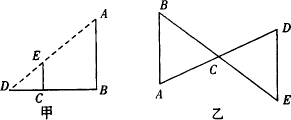
\includegraphics[width=2.51389in,height=0.90278in]{image35.png}

\textbf{1、定义:}三个角对应相等,三边对应成比例的两个三角形叫相似三角形,相似比记为

∽,则

\textbf{★2、性质:} ①相似三角形的对应角相等,对应边成比例;

②对应高的比、对应中线的比、对应角平分线的比、周长的比都等于相似比;

③相似三角形面积比等于相似比的平方。

\textbf{★3、判定:} ①两个角对应相等,两个三角形相似。

②两边对应成比例且夹角相等,两个三角形相似.

③三边对应成比例,两个三角形相似。

\textbf{★4、常见的相似模型}

\begin{longtable}[]{@{}lll@{}}
\toprule
\endhead
& &\tabularnewline
& 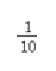
\includegraphics[width=1in,height=0.98611in]{image36.emf}
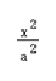
\includegraphics[width=1.09722in,height=0.98611in]{image37.emf}
&\tabularnewline
&
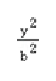
\includegraphics[width=2.38958in,height=1.06597in]{image38.emf}
&\tabularnewline
&
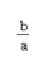
\includegraphics[width=1.23611in,height=0.79167in]{image39.emf}
\includegraphics[width=1.34722in,height=0.86111in]{image40.emf}
&\tabularnewline
&
\includegraphics[width=1.06944in,height=0.95833in]{image41.png}
\includegraphics[width=1.33333in,height=0.90278in]{image42.png}
&\tabularnewline
\bottomrule
\end{longtable}

\hypertarget{ux56dbux8fb9ux5f62}{%
\subsection{\texorpdfstring{
四边形}{ 四边形}}\label{ux56dbux8fb9ux5f62}}

\hypertarget{ux5b66ux79d1ux7f51www.zxxk.com--ux6559ux80b2ux8d44ux6e90ux95e8ux6237ux63d0ux4f9bux8bd5ux9898ux8bd5ux5377ux6559ux6848ux8bfeux4ef6ux6559ux5b66ux8bbaux6587ux7d20ux6750ux7b49ux5404ux7c7bux6559ux5b66ux8d44ux6e90ux5e93ux4e0bux8f7dux8fd8ux6709ux5927ux91cfux4e30ux5bccux7684ux6559ux5b66ux8d44ux8baf-12}{%
\subsubsection{\texorpdfstring{\protect\includegraphics[width=1.75in,height=0.34722in]{image5.png}}{学科网(www.zxxk.com)-\/-教育资源门户,提供试题试卷、教案、课件、教学论文、素材等各类教学资源库下载,还有大量丰富的教学资讯!}}\label{ux5b66ux79d1ux7f51www.zxxk.com--ux6559ux80b2ux8d44ux6e90ux95e8ux6237ux63d0ux4f9bux8bd5ux9898ux8bd5ux5377ux6559ux6848ux8bfeux4ef6ux6559ux5b66ux8bbaux6587ux7d20ux6750ux7b49ux5404ux7c7bux6559ux5b66ux8d44ux6e90ux5e93ux4e0bux8f7dux8fd8ux6709ux5927ux91cfux4e30ux5bccux7684ux6559ux5b66ux8d44ux8baf-12}}

\textbf{1、平行四边形性质与判定}

\begin{longtable}[]{@{}llll@{}}
\toprule
\endhead
&
\includegraphics[width=1.20833in,height=0.58333in]{image43.png}
& 定义 & 两组对边分别平行的四边形叫做平行四边形\tabularnewline
\begin{minipage}[t]{0.22\columnwidth}\raggedright
\strut
\end{minipage} & \begin{minipage}[t]{0.22\columnwidth}\raggedright
\strut
\end{minipage} & \begin{minipage}[t]{0.22\columnwidth}\raggedright
性质\strut
\end{minipage} & \begin{minipage}[t]{0.22\columnwidth}\raggedright
①对边平行且相等、对角相等、对角线互相平分、邻角互补

②\strut
\end{minipage}\tabularnewline
\begin{minipage}[t]{0.22\columnwidth}\raggedright
\strut
\end{minipage} & \begin{minipage}[t]{0.22\columnwidth}\raggedright
\strut
\end{minipage} & \begin{minipage}[t]{0.22\columnwidth}\raggedright
判定\strut
\end{minipage} & \begin{minipage}[t]{0.22\columnwidth}\raggedright
①一组对边平行且相等的四边形是平行四边形;

②两组对边分别相等(平行)的四边形是平行四边形;

③两组对角分别相等的四边形是平行四边形。\strut
\end{minipage}\tabularnewline
&
\includegraphics[width=1.25in,height=0.80556in]{image44.png}
& 定义 & 有一个角为的平行四边形叫做矩形\tabularnewline
\begin{minipage}[t]{0.22\columnwidth}\raggedright
\strut
\end{minipage} & \begin{minipage}[t]{0.22\columnwidth}\raggedright
\strut
\end{minipage} & \begin{minipage}[t]{0.22\columnwidth}\raggedright
性质\strut
\end{minipage} & \begin{minipage}[t]{0.22\columnwidth}\raggedright
①对角线相等、3个内角为直角

②\strut
\end{minipage}\tabularnewline
\begin{minipage}[t]{0.22\columnwidth}\raggedright
\strut
\end{minipage} & \begin{minipage}[t]{0.22\columnwidth}\raggedright
\strut
\end{minipage} & \begin{minipage}[t]{0.22\columnwidth}\raggedright
判定\strut
\end{minipage} & \begin{minipage}[t]{0.22\columnwidth}\raggedright
①有一(三)个角是直角的平行四边形(四边形)是矩形;

②对角线相等的平行四边形是矩形。\strut
\end{minipage}\tabularnewline
&
\includegraphics[width=1.22222in,height=0.77778in]{image45.png}
& 定义 & 有一组邻边相等的平行四边形叫做菱形\tabularnewline
\begin{minipage}[t]{0.22\columnwidth}\raggedright
\strut
\end{minipage} & \begin{minipage}[t]{0.22\columnwidth}\raggedright
\strut
\end{minipage} & \begin{minipage}[t]{0.22\columnwidth}\raggedright
性质\strut
\end{minipage} & \begin{minipage}[t]{0.22\columnwidth}\raggedright
①四边相等、\textbf{对角线平分对角}

②对角线互相垂直且平分

③菱形面积 = 对角线乘积的一半\strut
\end{minipage}\tabularnewline
\begin{minipage}[t]{0.22\columnwidth}\raggedright
\strut
\end{minipage} & \begin{minipage}[t]{0.22\columnwidth}\raggedright
\strut
\end{minipage} & \begin{minipage}[t]{0.22\columnwidth}\raggedright
判定\strut
\end{minipage} & \begin{minipage}[t]{0.22\columnwidth}\raggedright
①有一组邻边(四边)相等的平行四边形(四边形)是菱形;

②对角线互相垂直的平行四边形是菱形;

③对角线平分对角的平行四边形是菱形。\strut
\end{minipage}\tabularnewline
&
\includegraphics[width=1.13889in,height=1.18056in]{image46.png}
& 定义 & 4条边相等4个角为直角的四边形叫做矩形\tabularnewline
\begin{minipage}[t]{0.22\columnwidth}\raggedright
\strut
\end{minipage} & \begin{minipage}[t]{0.22\columnwidth}\raggedright
\strut
\end{minipage} & \begin{minipage}[t]{0.22\columnwidth}\raggedright
性质\strut
\end{minipage} & \begin{minipage}[t]{0.22\columnwidth}\raggedright
①四边相等,四个角都为

②对角线互相垂直、相等且互相平分。

③边长×边长\textbf{=×}对角线×对角线\strut
\end{minipage}\tabularnewline
\begin{minipage}[t]{0.22\columnwidth}\raggedright
\strut
\end{minipage} & \begin{minipage}[t]{0.22\columnwidth}\raggedright
\strut
\end{minipage} & \begin{minipage}[t]{0.22\columnwidth}\raggedright
判定\strut
\end{minipage} & \begin{minipage}[t]{0.22\columnwidth}\raggedright
①对角线垂直且相等的平行四边形是正方形

②邻边相等(对角线互相垂直)的矩形是正方形

③有一个角是直角(对角线相等)的菱形是正方形\strut
\end{minipage}\tabularnewline
\bottomrule
\end{longtable}

\hypertarget{ux601dux8defux603bux7ed3}{%
\subsubsection{\texorpdfstring{\textbf{2、思路总结}}{2、思路总结}}\label{ux601dux8defux603bux7ed3}}

\includegraphics[width=3.98611in,height=1.25in]{image47.png}

\textbf{3、平行四边形面积模型}

\begin{longtable}[]{@{}llll@{}}
\toprule
\endhead
\begin{minipage}[t]{0.22\columnwidth}\raggedright
\hypertarget{section-1}{%
\subsubsection{}\label{section-1}}\strut
\end{minipage} & \begin{minipage}[t]{0.22\columnwidth}\raggedright
\hypertarget{section-2}{%
\subsubsection{}\label{section-2}}\strut
\end{minipage} & \begin{minipage}[t]{0.22\columnwidth}\raggedright
\hypertarget{section-3}{%
\subsubsection{}\label{section-3}}\strut
\end{minipage} & \begin{minipage}[t]{0.22\columnwidth}\raggedright
\hypertarget{section-4}{%
\subsubsection{}\label{section-4}}\strut
\end{minipage}\tabularnewline
\begin{minipage}[t]{0.22\columnwidth}\raggedright
\hypertarget{section-5}{%
\subsubsection{}\label{section-5}}

\hypertarget{section-6}{%
\subsubsection{}\label{section-6}}\strut
\end{minipage} & \begin{minipage}[t]{0.22\columnwidth}\raggedright
\hypertarget{ux5e73ux884cux56dbux8fb9ux5f62ux8fb9ux4e0aux4e00ux70b9ux4e0eux4e24ux5bf9ux8fb9ux5f62ux6210ux7684ux4e24ux4e2aux4e09ux89d2ux5f62ux9762ux79efux548cux7b49ux4e8eux5e73ux884cux56dbux8fb9ux5f62ux9762ux79efux4e00ux534a}{%
\subsubsection{平行四边形边上一点与两对边形成的两个三角形面积和等于平行四边形面积一半。}\label{ux5e73ux884cux56dbux8fb9ux5f62ux8fb9ux4e0aux4e00ux70b9ux4e0eux4e24ux5bf9ux8fb9ux5f62ux6210ux7684ux4e24ux4e2aux4e09ux89d2ux5f62ux9762ux79efux548cux7b49ux4e8eux5e73ux884cux56dbux8fb9ux5f62ux9762ux79efux4e00ux534a}}\strut
\end{minipage} & \begin{minipage}[t]{0.22\columnwidth}\raggedright
\hypertarget{section-7}{%
\subsubsection{\texorpdfstring{\textbf{①}}{①}}\label{section-7}}

\hypertarget{section-8}{%
\subsubsection{\texorpdfstring{\textbf{②}}{②}}\label{section-8}}\strut
\end{minipage} & \begin{minipage}[t]{0.22\columnwidth}\raggedright
\hypertarget{ux5b66ux79d1ux7f51www.zxxk.com--ux6559ux80b2ux8d44ux6e90ux95e8ux6237ux63d0ux4f9bux8bd5ux9898ux8bd5ux5377ux6559ux6848ux8bfeux4ef6ux6559ux5b66ux8bbaux6587ux7d20ux6750ux7b49ux5404ux7c7bux6559ux5b66ux8d44ux6e90ux5e93ux4e0bux8f7dux8fd8ux6709ux5927ux91cfux4e30ux5bccux7684ux6559ux5b66ux8d44ux8baf-13}{%
\subsubsection{\texorpdfstring{\protect\includegraphics[width=1.69444in,height=0.77778in]{image48.png}}{学科网(www.zxxk.com)-\/-教育资源门户,提供试题试卷、教案、课件、教学论文、素材等各类教学资源库下载,还有大量丰富的教学资讯!}}\label{ux5b66ux79d1ux7f51www.zxxk.com--ux6559ux80b2ux8d44ux6e90ux95e8ux6237ux63d0ux4f9bux8bd5ux9898ux8bd5ux5377ux6559ux6848ux8bfeux4ef6ux6559ux5b66ux8bbaux6587ux7d20ux6750ux7b49ux5404ux7c7bux6559ux5b66ux8d44ux6e90ux5e93ux4e0bux8f7dux8fd8ux6709ux5927ux91cfux4e30ux5bccux7684ux6559ux5b66ux8d44ux8baf-13}}\strut
\end{minipage}\tabularnewline
\begin{minipage}[t]{0.22\columnwidth}\raggedright
\hypertarget{section-9}{%
\subsubsection{}\label{section-9}}

\hypertarget{section-10}{%
\subsubsection{}\label{section-10}}\strut
\end{minipage} & \begin{minipage}[t]{0.22\columnwidth}\raggedright
\hypertarget{ux5e73ux884cux56dbux8fb9ux5f62ux5185ux4e00ux70b9ux4e0eux4e24ux5bf9ux8fb9ux5f62ux6210ux7684ux4e24ux4e2aux4e09ux89d2ux5f62ux9762ux79efux548cux7b49ux4e8eux5e73ux884cux56dbux8fb9ux5f62ux9762ux79efux4e00ux534a}{%
\subsubsection{平行四边形内一点与两对边形成的两个三角形面积和等于平行四边形面积一半。}\label{ux5e73ux884cux56dbux8fb9ux5f62ux5185ux4e00ux70b9ux4e0eux4e24ux5bf9ux8fb9ux5f62ux6210ux7684ux4e24ux4e2aux4e09ux89d2ux5f62ux9762ux79efux548cux7b49ux4e8eux5e73ux884cux56dbux8fb9ux5f62ux9762ux79efux4e00ux534a}}\strut
\end{minipage} & \begin{minipage}[t]{0.22\columnwidth}\raggedright
\hypertarget{section-11}{%
\subsubsection{\texorpdfstring{\textbf{①}}{①}}\label{section-11}}

\hypertarget{section-12}{%
\subsubsection{\texorpdfstring{\textbf{②}}{②}}\label{section-12}}\strut
\end{minipage} & \begin{minipage}[t]{0.22\columnwidth}\raggedright
\hypertarget{ux5b66ux79d1ux7f51www.zxxk.com--ux6559ux80b2ux8d44ux6e90ux95e8ux6237ux63d0ux4f9bux8bd5ux9898ux8bd5ux5377ux6559ux6848ux8bfeux4ef6ux6559ux5b66ux8bbaux6587ux7d20ux6750ux7b49ux5404ux7c7bux6559ux5b66ux8d44ux6e90ux5e93ux4e0bux8f7dux8fd8ux6709ux5927ux91cfux4e30ux5bccux7684ux6559ux5b66ux8d44ux8baf-14}{%
\subsubsection{\texorpdfstring{\protect\includegraphics[width=1.625in,height=0.68056in]{image49.png}}{学科网(www.zxxk.com)-\/-教育资源门户,提供试题试卷、教案、课件、教学论文、素材等各类教学资源库下载,还有大量丰富的教学资讯!}}\label{ux5b66ux79d1ux7f51www.zxxk.com--ux6559ux80b2ux8d44ux6e90ux95e8ux6237ux63d0ux4f9bux8bd5ux9898ux8bd5ux5377ux6559ux6848ux8bfeux4ef6ux6559ux5b66ux8bbaux6587ux7d20ux6750ux7b49ux5404ux7c7bux6559ux5b66ux8d44ux6e90ux5e93ux4e0bux8f7dux8fd8ux6709ux5927ux91cfux4e30ux5bccux7684ux6559ux5b66ux8d44ux8baf-14}}\strut
\end{minipage}\tabularnewline
\begin{minipage}[t]{0.22\columnwidth}\raggedright
\hypertarget{section-13}{%
\subsubsection{}\label{section-13}}

\hypertarget{section-14}{%
\subsubsection{}\label{section-14}}\strut
\end{minipage} & \begin{minipage}[t]{0.22\columnwidth}\raggedright
\hypertarget{ux5e73ux884cux56dbux8fb9ux5f62ux5916ux4e00ux70b9ux4e0eux4e24ux5bf9ux8fb9ux5f62ux6210ux7684ux4e24ux4e2aux4e09ux89d2ux5f62ux9762ux79efux548cux5deeux4e3aux5e73ux884cux56dbux8fb9ux5f62ux9762ux79efux4e00ux534a}{%
\subsubsection{平行四边形外一点与两对边形成的两个三角形面积和(差)为平行四边形面积一半。}\label{ux5e73ux884cux56dbux8fb9ux5f62ux5916ux4e00ux70b9ux4e0eux4e24ux5bf9ux8fb9ux5f62ux6210ux7684ux4e24ux4e2aux4e09ux89d2ux5f62ux9762ux79efux548cux5deeux4e3aux5e73ux884cux56dbux8fb9ux5f62ux9762ux79efux4e00ux534a}}\strut
\end{minipage} & \begin{minipage}[t]{0.22\columnwidth}\raggedright
\hypertarget{section-15}{%
\subsubsection{\texorpdfstring{\textbf{①}}{①}}\label{section-15}}

\hypertarget{section-16}{%
\subsubsection{\texorpdfstring{\textbf{②}}{②}}\label{section-16}}\strut
\end{minipage} & \begin{minipage}[t]{0.22\columnwidth}\raggedright
\hypertarget{ux5b66ux79d1ux7f51www.zxxk.com--ux6559ux80b2ux8d44ux6e90ux95e8ux6237ux63d0ux4f9bux8bd5ux9898ux8bd5ux5377ux6559ux6848ux8bfeux4ef6ux6559ux5b66ux8bbaux6587ux7d20ux6750ux7b49ux5404ux7c7bux6559ux5b66ux8d44ux6e90ux5e93ux4e0bux8f7dux8fd8ux6709ux5927ux91cfux4e30ux5bccux7684ux6559ux5b66ux8d44ux8baf-15}{%
\subsubsection{\texorpdfstring{\protect\includegraphics[width=1.54167in,height=0.95833in]{image50.png}}{学科网(www.zxxk.com)-\/-教育资源门户,提供试题试卷、教案、课件、教学论文、素材等各类教学资源库下载,还有大量丰富的教学资讯!}}\label{ux5b66ux79d1ux7f51www.zxxk.com--ux6559ux80b2ux8d44ux6e90ux95e8ux6237ux63d0ux4f9bux8bd5ux9898ux8bd5ux5377ux6559ux6848ux8bfeux4ef6ux6559ux5b66ux8bbaux6587ux7d20ux6750ux7b49ux5404ux7c7bux6559ux5b66ux8d44ux6e90ux5e93ux4e0bux8f7dux8fd8ux6709ux5927ux91cfux4e30ux5bccux7684ux6559ux5b66ux8d44ux8baf-15}}\strut
\end{minipage}\tabularnewline
\bottomrule
\end{longtable}

\hypertarget{ux5b66ux79d1ux7f51www.zxxk.com--ux6559ux80b2ux8d44ux6e90ux95e8ux6237ux63d0ux4f9bux8bd5ux9898ux8bd5ux5377ux6559ux6848ux8bfeux4ef6ux6559ux5b66ux8bbaux6587ux7d20ux6750ux7b49ux5404ux7c7bux6559ux5b66ux8d44ux6e90ux5e93ux4e0bux8f7dux8fd8ux6709ux5927ux91cfux4e30ux5bccux7684ux6559ux5b66ux8d44ux8baf-16}{%
\subsubsection{\texorpdfstring{\protect\includegraphics[width=1.75in,height=0.34722in]{image5.png}}{学科网(www.zxxk.com)-\/-教育资源门户,提供试题试卷、教案、课件、教学论文、素材等各类教学资源库下载,还有大量丰富的教学资讯!}}\label{ux5b66ux79d1ux7f51www.zxxk.com--ux6559ux80b2ux8d44ux6e90ux95e8ux6237ux63d0ux4f9bux8bd5ux9898ux8bd5ux5377ux6559ux6848ux8bfeux4ef6ux6559ux5b66ux8bbaux6587ux7d20ux6750ux7b49ux5404ux7c7bux6559ux5b66ux8d44ux6e90ux5e93ux4e0bux8f7dux8fd8ux6709ux5927ux91cfux4e30ux5bccux7684ux6559ux5b66ux8d44ux8baf-16}}

\begin{longtable}[]{@{}lll@{}}
\toprule
\endhead
&
定义:任意画一个四边形,以四边的中点为顶点组成一个新四边形,这个新四边形就叫做原四边形的中点四边形.如下图点分别是四边形的边、、、的中点;
&\tabularnewline
& 对于任意四边形,四边形是平行四边形. &
\includegraphics[width=1.20833in,height=0.70833in]{image51.png}\tabularnewline
& 若对角线,则四边形是矩形. &
\includegraphics[width=1.29167in,height=0.75in]{image52.png}\tabularnewline
& 若对角线,则四边形是菱形. &
\includegraphics[width=1.40278in,height=0.68056in]{image53.png}\tabularnewline
& 对角线且,则四边形是正方形. &
\includegraphics[width=1.06944in,height=0.93056in]{image54.png}\tabularnewline
\bottomrule
\end{longtable}

\hypertarget{ux5706}{%
\subsection{\texorpdfstring{ 圆}{ 圆}}\label{ux5706}}

\hypertarget{ux5b66ux79d1ux7f51www.zxxk.com--ux6559ux80b2ux8d44ux6e90ux95e8ux6237ux63d0ux4f9bux8bd5ux9898ux8bd5ux5377ux6559ux6848ux8bfeux4ef6ux6559ux5b66ux8bbaux6587ux7d20ux6750ux7b49ux5404ux7c7bux6559ux5b66ux8d44ux6e90ux5e93ux4e0bux8f7dux8fd8ux6709ux5927ux91cfux4e30ux5bccux7684ux6559ux5b66ux8d44ux8baf-17}{%
\subsubsection{\texorpdfstring{\protect\includegraphics[width=1.75in,height=0.34722in]{image5.png}}{学科网(www.zxxk.com)-\/-教育资源门户,提供试题试卷、教案、课件、教学论文、素材等各类教学资源库下载,还有大量丰富的教学资讯!}}\label{ux5b66ux79d1ux7f51www.zxxk.com--ux6559ux80b2ux8d44ux6e90ux95e8ux6237ux63d0ux4f9bux8bd5ux9898ux8bd5ux5377ux6559ux6848ux8bfeux4ef6ux6559ux5b66ux8bbaux6587ux7d20ux6750ux7b49ux5404ux7c7bux6559ux5b66ux8d44ux6e90ux5e93ux4e0bux8f7dux8fd8ux6709ux5927ux91cfux4e30ux5bccux7684ux6559ux5b66ux8d44ux8baf-17}}

\begin{longtable}[]{@{}lll@{}}
\toprule
\endhead
& &\tabularnewline
&
在一个平面内,线段绕它固定的一个端点旋转一周,另一个端点所形成的图形叫做圆.圆是轴对称图形,也是中心对称图形,其对称轴是任意一条过原点的直线,对称中心是圆心。圆用⊙表示,半径为
&
\includegraphics[width=1.09722in,height=1.01389in]{image55.emf}\tabularnewline
\begin{minipage}[t]{0.30\columnwidth}\raggedright
\strut
\end{minipage} & \begin{minipage}[t]{0.30\columnwidth}\raggedright
弦:连接圆上任意两点的线段叫做弦.经过圆心的弦叫做直径,并且直径是同一圆中最长的弦。

弧:圆上任意两点间的部分叫做圆弧,简称弧。在一个圆中大于半圆的弧叫做优弧,小于半圆的弧叫做劣弧。\strut
\end{minipage} & \begin{minipage}[t]{0.30\columnwidth}\raggedright
\includegraphics[width=1.54167in,height=0.98611in]{image56.emf}\strut
\end{minipage}\tabularnewline
\begin{minipage}[t]{0.30\columnwidth}\raggedright
\strut
\end{minipage} & \begin{minipage}[t]{0.30\columnwidth}\raggedright
圆心角:顶点在圆心的角叫做圆心角。

圆周角:顶点在圆上,并且两边都和圆相交的角叫做圆周角。\strut
\end{minipage} & \begin{minipage}[t]{0.30\columnwidth}\raggedright
\includegraphics[width=1in,height=0.875in]{image57.emf}\strut
\end{minipage}\tabularnewline
\begin{minipage}[t]{0.30\columnwidth}\raggedright
\strut
\end{minipage} & \begin{minipage}[t]{0.30\columnwidth}\raggedright
扇形:一条弧和经过这条弧两端的两条半径所围成的图形叫扇形。

弓形:由弦及其所对的弧组成的图形叫做弓形。\strut
\end{minipage} & \begin{minipage}[t]{0.30\columnwidth}\raggedright
\includegraphics[width=0.76389in,height=0.75in]{image58.png}\strut
\end{minipage}\tabularnewline
\begin{minipage}[t]{0.30\columnwidth}\raggedright
\strut
\end{minipage} & \begin{minipage}[t]{0.30\columnwidth}\raggedright
垂径定理:垂直于弦的直径平分这条弦,并且平分弦所对的两条弧。

推论:平分弦的直径垂直于弦,并且平分弦所对的两条弧。\strut
\end{minipage} & \begin{minipage}[t]{0.30\columnwidth}\raggedright
\includegraphics[width=0.97222in,height=0.94444in]{image59.png}\strut
\end{minipage}\tabularnewline
\bottomrule
\end{longtable}

\hypertarget{section-17}{%
\subsubsection{}\label{section-17}}

\hypertarget{ux5b66ux79d1ux7f51www.zxxk.com--ux6559ux80b2ux8d44ux6e90ux95e8ux6237ux63d0ux4f9bux8bd5ux9898ux8bd5ux5377ux6559ux6848ux8bfeux4ef6ux6559ux5b66ux8bbaux6587ux7d20ux6750ux7b49ux5404ux7c7bux6559ux5b66ux8d44ux6e90ux5e93ux4e0bux8f7dux8fd8ux6709ux5927ux91cfux4e30ux5bccux7684ux6559ux5b66ux8d44ux8baf-18}{%
\subsubsection{\texorpdfstring{\protect\includegraphics[width=1.88889in,height=0.34722in]{image5.png}}{学科网(www.zxxk.com)-\/-教育资源门户,提供试题试卷、教案、课件、教学论文、素材等各类教学资源库下载,还有大量丰富的教学资讯!}}\label{ux5b66ux79d1ux7f51www.zxxk.com--ux6559ux80b2ux8d44ux6e90ux95e8ux6237ux63d0ux4f9bux8bd5ux9898ux8bd5ux5377ux6559ux6848ux8bfeux4ef6ux6559ux5b66ux8bbaux6587ux7d20ux6750ux7b49ux5404ux7c7bux6559ux5b66ux8d44ux6e90ux5e93ux4e0bux8f7dux8fd8ux6709ux5927ux91cfux4e30ux5bccux7684ux6559ux5b66ux8d44ux8baf-18}}

\begin{longtable}[]{@{}lll@{}}
\toprule
\endhead
& &\tabularnewline
&
在同圆或等圆中,相等的圆心角所对的弧相等,所对的弦相等,所对的弦心距也相等。
&
\includegraphics[width=0.875in,height=0.84722in]{image60.png}\tabularnewline
\begin{minipage}[t]{0.30\columnwidth}\raggedright
\strut
\end{minipage} & \begin{minipage}[t]{0.30\columnwidth}\raggedright
定理:在同圆或等圆中,同弧或等弧所对的圆周角都相等,且都等于它所对的圆心角的一半。

如图:\strut
\end{minipage} & \begin{minipage}[t]{0.30\columnwidth}\raggedright
\includegraphics[width=0.97222in,height=1.04167in]{image61.png}\strut
\end{minipage}\tabularnewline
\begin{minipage}[t]{0.30\columnwidth}\raggedright
\strut
\end{minipage} & \begin{minipage}[t]{0.30\columnwidth}\raggedright
推论1:半圆(或直径)所对的圆周角是直角,的圆周角所对的弧(或弦)是半圆(或直径)。

如图:\strut
\end{minipage} & \begin{minipage}[t]{0.30\columnwidth}\raggedright
\includegraphics[width=1.06944in,height=0.90278in]{image62.png}\strut
\end{minipage}\tabularnewline
\begin{minipage}[t]{0.30\columnwidth}\raggedright
\strut
\end{minipage} & \begin{minipage}[t]{0.30\columnwidth}\raggedright
推论2:圆内接四边形的对角互补。

如图:,.\strut
\end{minipage} & \begin{minipage}[t]{0.30\columnwidth}\raggedright
\includegraphics[width=1.11111in,height=0.86111in]{image63.emf}\strut
\end{minipage}\tabularnewline
\bottomrule
\end{longtable}

\hypertarget{section-18}{%
\subsubsection{}\label{section-18}}

\hypertarget{ux5b66ux79d1ux7f51www.zxxk.com--ux6559ux80b2ux8d44ux6e90ux95e8ux6237ux63d0ux4f9bux8bd5ux9898ux8bd5ux5377ux6559ux6848ux8bfeux4ef6ux6559ux5b66ux8bbaux6587ux7d20ux6750ux7b49ux5404ux7c7bux6559ux5b66ux8d44ux6e90ux5e93ux4e0bux8f7dux8fd8ux6709ux5927ux91cfux4e30ux5bccux7684ux6559ux5b66ux8d44ux8baf-19}{%
\subsubsection{\texorpdfstring{\protect\includegraphics[width=1.75in,height=0.34722in]{image5.png}}{学科网(www.zxxk.com)-\/-教育资源门户,提供试题试卷、教案、课件、教学论文、素材等各类教学资源库下载,还有大量丰富的教学资讯!}}\label{ux5b66ux79d1ux7f51www.zxxk.com--ux6559ux80b2ux8d44ux6e90ux95e8ux6237ux63d0ux4f9bux8bd5ux9898ux8bd5ux5377ux6559ux6848ux8bfeux4ef6ux6559ux5b66ux8bbaux6587ux7d20ux6750ux7b49ux5404ux7c7bux6559ux5b66ux8d44ux6e90ux5e93ux4e0bux8f7dux8fd8ux6709ux5927ux91cfux4e30ux5bccux7684ux6559ux5b66ux8d44ux8baf-19}}

\textbf{1、直线和圆的关系}

\begin{longtable}[]{@{}llll@{}}
\toprule
\endhead
& & &\tabularnewline
直线与⊙相交 & 直线与圆有两个交点,直线叫做圆的割线。 & &\tabularnewline
直线与⊙相切 & 直线与圆有唯一交点,直线叫做圆的切线,交点叫做圆的切点。 &
&\tabularnewline
直线与⊙相离 & 直线与圆没有交点。 & &\tabularnewline
\bottomrule
\end{longtable}

\textbf{★2、切线判定定理}

定理:经过半径的外端并且垂直于这条半径的直线是圆的切线。

根据圆的切线判定定理,以后在题中证明圆的切线,连半径,证垂直。

\textbf{★3、切线长定理:}

切线长:过圆外一点作圆的切线,这点和切点间线段的长,叫点到圆的切线长.

切线长定理:过圆外一点所画的圆的两条切线长相等,并且这点和圆心的连线

平分两条切线的夹角.

如图所示,、分别与⊙切于点、,则,平分.

\includegraphics[width=1in,height=1.05556in]{image24.png}

\textbf{4、三角形的外接圆}

①确定圆的条件:不在同一直线上的三点确定一个圆.

②外接圆定义:经过三角形三个顶点的圆叫做三角形的外接圆,外接圆的

圆心是三角形三条边垂直平分线的交点,叫做三角形的外心,这个三角形叫

做这个圆的内接三角形.

\textbf{5、三角形的内切圆}

和三角形各边都相切的圆叫做三角形的内切圆,内切圆的圆心叫做三角形的

内心,内心是三条内角平分线的交点.

\hypertarget{ux5b66ux79d1ux7f51www.zxxk.com--ux6559ux80b2ux8d44ux6e90ux95e8ux6237ux63d0ux4f9bux8bd5ux9898ux8bd5ux5377ux6559ux6848ux8bfeux4ef6ux6559ux5b66ux8bbaux6587ux7d20ux6750ux7b49ux5404ux7c7bux6559ux5b66ux8d44ux6e90ux5e93ux4e0bux8f7dux8fd8ux6709ux5927ux91cfux4e30ux5bccux7684ux6559ux5b66ux8d44ux8baf-20}{%
\subsubsection{\texorpdfstring{\protect\includegraphics[width=1.75in,height=0.34722in]{image5.png}}{学科网(www.zxxk.com)-\/-教育资源门户,提供试题试卷、教案、课件、教学论文、素材等各类教学资源库下载,还有大量丰富的教学资讯!}}\label{ux5b66ux79d1ux7f51www.zxxk.com--ux6559ux80b2ux8d44ux6e90ux95e8ux6237ux63d0ux4f9bux8bd5ux9898ux8bd5ux5377ux6559ux6848ux8bfeux4ef6ux6559ux5b66ux8bbaux6587ux7d20ux6750ux7b49ux5404ux7c7bux6559ux5b66ux8d44ux6e90ux5e93ux4e0bux8f7dux8fd8ux6709ux5927ux91cfux4e30ux5bccux7684ux6559ux5b66ux8d44ux8baf-20}}

\begin{longtable}[]{@{}lll@{}}
\toprule
\endhead
& &\tabularnewline
\begin{minipage}[t]{0.30\columnwidth}\raggedright
\strut
\end{minipage} & \begin{minipage}[t]{0.30\columnwidth}\raggedright
弦切角:切线与弦的夹角。

弦切角定理:弦切角等于它所夹弧的圆周角。

如图:.\strut
\end{minipage} & \begin{minipage}[t]{0.30\columnwidth}\raggedright
\includegraphics[width=1.26389in,height=0.76389in]{image68.png}\strut
\end{minipage}\tabularnewline
& 相交弦定理:圆内的两条相交弦被交点分成的两条线段长乘积相等。如图:.
&\tabularnewline
\begin{minipage}[t]{0.30\columnwidth}\raggedright
\strut
\end{minipage} & \begin{minipage}[t]{0.30\columnwidth}\raggedright
切割线定理:从圆外一点引圆的切线和割线,切线长是这点到割线与圆交点的两条线段长的比例中项。

如图:.\strut
\end{minipage} & \begin{minipage}[t]{0.30\columnwidth}\raggedright
\strut
\end{minipage}\tabularnewline
\begin{minipage}[t]{0.30\columnwidth}\raggedright
\strut
\end{minipage} & \begin{minipage}[t]{0.30\columnwidth}\raggedright
割线定理:从圆外一点引圆的两条割线,这一点到每条割线与圆的交点的两条线段长的积相等。

如图:.\strut
\end{minipage} & \begin{minipage}[t]{0.30\columnwidth}\raggedright
\strut
\end{minipage}\tabularnewline
\bottomrule
\end{longtable}

\hypertarget{section-19}{%
\subsubsection{}\label{section-19}}

\hypertarget{ux5b66ux79d1ux7f51www.zxxk.com--ux6559ux80b2ux8d44ux6e90ux95e8ux6237ux63d0ux4f9bux8bd5ux9898ux8bd5ux5377ux6559ux6848ux8bfeux4ef6ux6559ux5b66ux8bbaux6587ux7d20ux6750ux7b49ux5404ux7c7bux6559ux5b66ux8d44ux6e90ux5e93ux4e0bux8f7dux8fd8ux6709ux5927ux91cfux4e30ux5bccux7684ux6559ux5b66ux8d44ux8baf-21}{%
\subsubsection{\texorpdfstring{\protect\includegraphics[width=1.75in,height=0.34722in]{image5.png}}{学科网(www.zxxk.com)-\/-教育资源门户,提供试题试卷、教案、课件、教学论文、素材等各类教学资源库下载,还有大量丰富的教学资讯!}}\label{ux5b66ux79d1ux7f51www.zxxk.com--ux6559ux80b2ux8d44ux6e90ux95e8ux6237ux63d0ux4f9bux8bd5ux9898ux8bd5ux5377ux6559ux6848ux8bfeux4ef6ux6559ux5b66ux8bbaux6587ux7d20ux6750ux7b49ux5404ux7c7bux6559ux5b66ux8d44ux6e90ux5e93ux4e0bux8f7dux8fd8ux6709ux5927ux91cfux4e30ux5bccux7684ux6559ux5b66ux8d44ux8baf-21}}

\begin{longtable}[]{@{}lll@{}}
\toprule
\endhead
& &\tabularnewline
& 弧长公式: &
\includegraphics[width=0.88889in,height=0.84722in]{image72.png}\tabularnewline
& 面积公式: &\tabularnewline
\begin{minipage}[t]{0.30\columnwidth}\raggedright
\strut
\end{minipage} & \begin{minipage}[t]{0.30\columnwidth}\raggedright
圆锥展开:侧面展开图是扇形,底面是圆。

为扇形半径,也叫圆锥母线长。\strut
\end{minipage} & \begin{minipage}[t]{0.30\columnwidth}\raggedright
\includegraphics[width=1.05556in,height=0.81944in]{image73.png}\strut
\end{minipage}\tabularnewline
\begin{minipage}[t]{0.30\columnwidth}\raggedright
\strut
\end{minipage} & \begin{minipage}[t]{0.30\columnwidth}\raggedright
圆锥个考点:

①侧面展开图中:扇形弧长=底面圆周长。即:

②在圆锥内由勾股定理有:\strut
\end{minipage} & \begin{minipage}[t]{0.30\columnwidth}\raggedright
\includegraphics[width=0.81944in,height=0.95833in]{image74.png}\strut
\end{minipage}\tabularnewline
& &\tabularnewline
\bottomrule
\end{longtable}

\hypertarget{ux65cbux8f6cux4e0eux89c6ux56fe}{%
\subsection{\texorpdfstring{
旋转与视图}{ 旋转与视图}}\label{ux65cbux8f6cux4e0eux89c6ux56fe}}

\hypertarget{ux5b66ux79d1ux7f51www.zxxk.com--ux6559ux80b2ux8d44ux6e90ux95e8ux6237ux63d0ux4f9bux8bd5ux9898ux8bd5ux5377ux6559ux6848ux8bfeux4ef6ux6559ux5b66ux8bbaux6587ux7d20ux6750ux7b49ux5404ux7c7bux6559ux5b66ux8d44ux6e90ux5e93ux4e0bux8f7dux8fd8ux6709ux5927ux91cfux4e30ux5bccux7684ux6559ux5b66ux8d44ux8baf-22}{%
\subsubsection{\texorpdfstring{\protect\includegraphics[width=1.75in,height=0.34722in]{image5.png}}{学科网(www.zxxk.com)-\/-教育资源门户,提供试题试卷、教案、课件、教学论文、素材等各类教学资源库下载,还有大量丰富的教学资讯!}}\label{ux5b66ux79d1ux7f51www.zxxk.com--ux6559ux80b2ux8d44ux6e90ux95e8ux6237ux63d0ux4f9bux8bd5ux9898ux8bd5ux5377ux6559ux6848ux8bfeux4ef6ux6559ux5b66ux8bbaux6587ux7d20ux6750ux7b49ux5404ux7c7bux6559ux5b66ux8d44ux6e90ux5e93ux4e0bux8f7dux8fd8ux6709ux5927ux91cfux4e30ux5bccux7684ux6559ux5b66ux8d44ux8baf-22}}

\begin{longtable}[]{@{}lll@{}}
\toprule
\endhead
& &\tabularnewline
&
把一个平面图形绕着平面内某一点转动一个角度,就叫做图形的旋转,点叫做旋转中心,转动的角叫做旋转角,如果图形上的点经过旋转变为点,那么这两个点叫做这个旋转的对应点。
&
\includegraphics[width=1.51389in,height=0.90278in]{image75.png}\tabularnewline
\begin{minipage}[t]{0.30\columnwidth}\raggedright
\strut
\end{minipage} & \begin{minipage}[t]{0.30\columnwidth}\raggedright
\textbf{(1)}旋转后的图形与原图形是全等的

\textbf{(2)}旋转前后两个图形对应点到旋转中心的距离相等

\textbf{(3)}对应点与旋转中心所连线段的夹角都是旋转角\strut
\end{minipage} & \begin{minipage}[t]{0.30\columnwidth}\raggedright
\includegraphics[width=1.38889in,height=1.68056in]{image76.png}\strut
\end{minipage}\tabularnewline
\begin{minipage}[t]{0.30\columnwidth}\raggedright
\strut
\end{minipage} & \begin{minipage}[t]{0.30\columnwidth}\raggedright
\textbf{(1)}首先确定旋转的三要素:\textbf{旋转中心、旋转方向、旋转角};

\textbf{(2)}其次在原图中找几个关键点;

\textbf{(3)}再连接关键点与旋转中心,让关键点与旋转中心所连线段沿旋转方向转动一定的角度,得到线段的端点就是关键点的对应点;

\textbf{(4)}最后依次连接各对应点,就得到旋转后的图形。\strut
\end{minipage} & \begin{minipage}[t]{0.30\columnwidth}\raggedright
\includegraphics[width=1.54167in,height=1.70833in]{image77.png}\strut
\end{minipage}\tabularnewline
&
定义:把一个图形绕着某一个点旋转180°,如果旋转后的图形能够与原来的图形重合,那么这个图形叫做中心对称图形,这个点叫做对称中心。
&
\includegraphics[width=0.61111in,height=0.625in]{image78.png}
\includegraphics[width=0.68056in,height=0.68056in]{image79.png}\tabularnewline
\begin{minipage}[t]{0.30\columnwidth}\raggedright
\strut
\end{minipage} & \begin{minipage}[t]{0.30\columnwidth}\raggedright
把一个图形沿着某一条直线折叠,如果它能够与另一个图形重合,那么就说这两个图形关于这条直线对称,两个图形中的对应点叫做对称点,对应线段叫做对称线段。

\textbf{轴对称性质:}①关于某条直线对称的两个图形是全等形;

②对称轴是任何一对对应点所连线的垂直平分线。\strut
\end{minipage} & \begin{minipage}[t]{0.30\columnwidth}\raggedright
\includegraphics[width=0.65278in,height=0.58333in]{image80.png}\strut
\end{minipage}\tabularnewline
\begin{minipage}[t]{0.30\columnwidth}\raggedright
\strut
\end{minipage} & \begin{minipage}[t]{0.30\columnwidth}\raggedright
(1)作出已知图各顶点关于对称轴(对称中心)的对称点------连接关键点和对称轴(对称中心),并延长\textbf{一倍}确定对称点.

(2)把各对称点按已知图形的连接方式依次连接起来,则所得到的图形就是已知图形关于对称轴(对称中心)对称的图形.\strut
\end{minipage} & \begin{minipage}[t]{0.30\columnwidth}\raggedright
\includegraphics[width=1.58333in,height=1.41667in]{image81.png}\strut
\end{minipage}\tabularnewline
\bottomrule
\end{longtable}

\hypertarget{ux5b66ux79d1ux7f51www.zxxk.com--ux6559ux80b2ux8d44ux6e90ux95e8ux6237ux63d0ux4f9bux8bd5ux9898ux8bd5ux5377ux6559ux6848ux8bfeux4ef6ux6559ux5b66ux8bbaux6587ux7d20ux6750ux7b49ux5404ux7c7bux6559ux5b66ux8d44ux6e90ux5e93ux4e0bux8f7dux8fd8ux6709ux5927ux91cfux4e30ux5bccux7684ux6559ux5b66ux8d44ux8baf-23}{%
\subsubsection{\texorpdfstring{\protect\includegraphics[width=1.75in,height=0.34722in]{image5.png}}{学科网(www.zxxk.com)-\/-教育资源门户,提供试题试卷、教案、课件、教学论文、素材等各类教学资源库下载,还有大量丰富的教学资讯!}}\label{ux5b66ux79d1ux7f51www.zxxk.com--ux6559ux80b2ux8d44ux6e90ux95e8ux6237ux63d0ux4f9bux8bd5ux9898ux8bd5ux5377ux6559ux6848ux8bfeux4ef6ux6559ux5b66ux8bbaux6587ux7d20ux6750ux7b49ux5404ux7c7bux6559ux5b66ux8d44ux6e90ux5e93ux4e0bux8f7dux8fd8ux6709ux5927ux91cfux4e30ux5bccux7684ux6559ux5b66ux8d44ux8baf-23}}

\textbf{1、投影与视图}

\begin{longtable}[]{@{}llll@{}}
\toprule
\endhead
& & &\tabularnewline
&
用平行光线(太阳光)照射物体,在某个平面(地面或墙壁等)上得到的投影叫做平行投影。
& 在同一时刻,不同物体的物高与影长成正比例. &
\includegraphics[width=1.66667in,height=0.83333in]{image82.png}\tabularnewline
&
用点光线(灯光)照射物体,在某个平面(地面或墙壁等)上得到的投影叫做中心投影。
& 中心投影中存在三角形相似 &
\includegraphics[width=1.22222in,height=0.81944in]{image83.png}\tabularnewline
\begin{minipage}[t]{0.22\columnwidth}\raggedright
\strut
\end{minipage} & \begin{minipage}[t]{0.22\columnwidth}\raggedright
一物体在三个投影面内进行正投影,在正面得到的的视图叫主视图;在水平面得到的叫俯视图;在侧面内得到的视图叫左视图.主视图、左视图、俯视图叫做物体的三视图.\strut
\end{minipage} & \begin{minipage}[t]{0.22\columnwidth}\raggedright
长对正

高平齐

宽相等\strut
\end{minipage} & \begin{minipage}[t]{0.22\columnwidth}\raggedright
\includegraphics[width=1.25in,height=1.26389in]{image84.png}\includegraphics[width=1.38889in,height=0.97222in]{image84.png}\strut
\end{minipage}\tabularnewline
\bottomrule
\end{longtable}

\textbf{★2、投影与视图的考点}

\begin{longtable}[]{@{}ll@{}}
\toprule
\endhead
\begin{minipage}[t]{0.47\columnwidth}\raggedright
\strut
\end{minipage} & \begin{minipage}[t]{0.47\columnwidth}\raggedright
\includegraphics[width=1.45556in,height=1.51042in]{image85.png}如图,小美利用所学的数学知识测量旗杆\includegraphics[width=0.23611in,height=0.15278in]{image86.png}的高度.

(1)画出此时旗杆\includegraphics[width=0.23611in,height=0.15278in]{image86.png}在阳光下的投影;

(2)已知小美的身高为\includegraphics[width=0.44444in,height=0.15278in]{image87.png},在同一时刻测得小美和旗杆AB的投影长分别为\includegraphics[width=0.44444in,height=0.15278in]{image88.png}和\includegraphics[width=0.23611in,height=0.15278in]{image89.png},求旗杆\includegraphics[width=0.23611in,height=0.15278in]{image86.png}的高.

解答:(1)如下图,假设小美为\includegraphics[width=0.23611in,height=0.125in]{image90.png},她的影子为\includegraphics[width=0.23611in,height=0.125in]{image91.png},

\includegraphics[width=1.49306in,height=1.32778in]{image92.png}连接\includegraphics[width=0.23611in,height=0.125in]{image93.png},过点\includegraphics[width=0.11111in,height=0.125in]{image94.png}作\includegraphics[width=0.61111in,height=0.16667in]{image95.png}交地面于点\includegraphics[width=0.125in,height=0.125in]{image96.png},

连接\includegraphics[width=0.23611in,height=0.125in]{image97.png},\includegraphics[width=0.23611in,height=0.125in]{image97.png}即为此时旗杆在阳光下的投影.

(2)由(1)可知,\includegraphics[width=0.23611in,height=0.125in]{image90.png},\includegraphics[width=0.23611in,height=0.125in]{image98.png}都垂直于地面,且\includegraphics[width=0.61111in,height=0.16667in]{image95.png},

\includegraphics[width=1.625in,height=0.15278in]{image99.png},\includegraphics[width=1.08333in,height=0.15278in]{image100.png},\includegraphics[width=1.27778in,height=0.15278in]{image101.png},\includegraphics[width=0.90278in,height=0.33333in]{image102.png}.由题可知\includegraphics[width=0.875in,height=0.15278in]{image103.png},\includegraphics[width=0.86111in,height=0.15278in]{image104.png},\includegraphics[width=0.65278in,height=0.15278in]{image105.png},\includegraphics[width=1in,height=0.33333in]{image106.png},解得\includegraphics[width=0.81944in,height=0.16667in]{image107.png},\includegraphics[width=0.11111in,height=0.11111in]{image108.png}旗杆\includegraphics[width=0.23611in,height=0.125in]{image98.png}的高为\includegraphics[width=0.31944in,height=0.15278in]{image109.png}.\strut
\end{minipage}\tabularnewline
\begin{minipage}[t]{0.47\columnwidth}\raggedright
\strut
\end{minipage} & \begin{minipage}[t]{0.47\columnwidth}\raggedright
\includegraphics[width=1.47431in,height=1.59444in]{image110.png}如图是一个几何体的三视图,则这个几何体是(
~ )

A.\includegraphics[width=0.69444in,height=0.61111in]{image111.png}B.\includegraphics[width=0.73611in,height=0.69444in]{image112.png}C.\includegraphics[width=0.70833in,height=0.66667in]{image113.png}D.\includegraphics[width=0.75in,height=0.70833in]{image114.png}

根据主视图、左视图、俯视图可知,该几何体为正方体缺少右前上的一块,故选\includegraphics[width=0.125in,height=0.15278in]{image115.png}.\strut
\end{minipage}\tabularnewline
\bottomrule
\end{longtable}

\hypertarget{ux51e0ux4f55ux89e3ux9898ux65b9ux6cd5ux4e0eux601dux8def}{%
\subsection{\texorpdfstring{
几何解题方法与思路}{ 几何解题方法与思路}}\label{ux51e0ux4f55ux89e3ux9898ux65b9ux6cd5ux4e0eux601dux8def}}

\hypertarget{ux5b66ux79d1ux7f51www.zxxk.com--ux6559ux80b2ux8d44ux6e90ux95e8ux6237ux63d0ux4f9bux8bd5ux9898ux8bd5ux5377ux6559ux6848ux8bfeux4ef6ux6559ux5b66ux8bbaux6587ux7d20ux6750ux7b49ux5404ux7c7bux6559ux5b66ux8d44ux6e90ux5e93ux4e0bux8f7dux8fd8ux6709ux5927ux91cfux4e30ux5bccux7684ux6559ux5b66ux8d44ux8baf-24}{%
\subsubsection{\texorpdfstring{\protect\includegraphics[width=1.75in,height=0.34722in]{image5.png}}{学科网(www.zxxk.com)-\/-教育资源门户,提供试题试卷、教案、课件、教学论文、素材等各类教学资源库下载,还有大量丰富的教学资讯!}}\label{ux5b66ux79d1ux7f51www.zxxk.com--ux6559ux80b2ux8d44ux6e90ux95e8ux6237ux63d0ux4f9bux8bd5ux9898ux8bd5ux5377ux6559ux6848ux8bfeux4ef6ux6559ux5b66ux8bbaux6587ux7d20ux6750ux7b49ux5404ux7c7bux6559ux5b66ux8d44ux6e90ux5e93ux4e0bux8f7dux8fd8ux6709ux5927ux91cfux4e30ux5bccux7684ux6559ux5b66ux8d44ux8baf-24}}

\begin{longtable}[]{@{}lll@{}}
\toprule
\endhead
& &\tabularnewline
& &\tabularnewline
& 作一个角与相等 &
\includegraphics[width=1.11111in,height=0.81944in]{image116.png}~\includegraphics[width=1.26389in,height=0.83333in]{image117.png}\tabularnewline
& 作的角平分线 &
\includegraphics[width=1.15278in,height=0.75in]{image118.png}\tabularnewline
\begin{minipage}[t]{0.30\columnwidth}\raggedright
\strut
\end{minipage} & \begin{minipage}[t]{0.30\columnwidth}\raggedright
作直线的垂线,使它经过点\strut
\end{minipage} & \begin{minipage}[t]{0.30\columnwidth}\raggedright
①点在线段上~~~~~

②点在线段外

\includegraphics[width=1.11111in,height=1.02778in]{image119.png}
\includegraphics[width=1.04167in,height=0.86111in]{image120.png}\strut
\end{minipage}\tabularnewline
& 作圆,使它经过不同一直线上的三点(即作以点为顶点的三角形的外接圆) &
\includegraphics[width=1.52778in,height=1.22222in]{image121.png}\tabularnewline
& 作以点为顶点的三角形的内切圆 &
\includegraphics[width=1.61111in,height=1.125in]{image122.png}\tabularnewline
\bottomrule
\end{longtable}

\hypertarget{section-20}{%
\subsubsection{}\label{section-20}}

\hypertarget{ux5b66ux79d1ux7f51www.zxxk.com--ux6559ux80b2ux8d44ux6e90ux95e8ux6237ux63d0ux4f9bux8bd5ux9898ux8bd5ux5377ux6559ux6848ux8bfeux4ef6ux6559ux5b66ux8bbaux6587ux7d20ux6750ux7b49ux5404ux7c7bux6559ux5b66ux8d44ux6e90ux5e93ux4e0bux8f7dux8fd8ux6709ux5927ux91cfux4e30ux5bccux7684ux6559ux5b66ux8d44ux8baf-25}{%
\subsubsection{\texorpdfstring{\protect\includegraphics[width=1.75in,height=0.34722in]{image5.png}}{学科网(www.zxxk.com)-\/-教育资源门户,提供试题试卷、教案、课件、教学论文、素材等各类教学资源库下载,还有大量丰富的教学资讯!}}\label{ux5b66ux79d1ux7f51www.zxxk.com--ux6559ux80b2ux8d44ux6e90ux95e8ux6237ux63d0ux4f9bux8bd5ux9898ux8bd5ux5377ux6559ux6848ux8bfeux4ef6ux6559ux5b66ux8bbaux6587ux7d20ux6750ux7b49ux5404ux7c7bux6559ux5b66ux8d44ux6e90ux5e93ux4e0bux8f7dux8fd8ux6709ux5927ux91cfux4e30ux5bccux7684ux6559ux5b66ux8d44ux8baf-25}}

\begin{longtable}[]{@{}lll@{}}
\toprule
\endhead
& &\tabularnewline
& \textbf{截长(在上截取一点,使得,可证得)} &
\includegraphics[width=1.09722in,height=0.58333in]{image123.png}\includegraphics[width=1.20833in,height=0.68056in]{image124.png}\tabularnewline
& \textbf{补短(延长到点,使得,连接,可证得)} &
\includegraphics[width=1.09722in,height=0.58333in]{image123.png}\includegraphics[width=1.33333in,height=0.94444in]{image125.png}\tabularnewline
& \textbf{斜边中线(斜边中线等于斜边一半,即)} &
\includegraphics[width=0.88889in,height=1.08333in]{image126.png}\includegraphics[width=0.93056in,height=1.11111in]{image26.png}\tabularnewline
& \textbf{三角形中位线(三角形中位线第三边,且等于第三边一半,即且)} &
\includegraphics[width=1.29167in,height=0.83333in]{image127.png}\includegraphics[width=1.22222in,height=0.81944in]{image128.png}\tabularnewline
\begin{minipage}[t]{0.30\columnwidth}\raggedright
\strut
\end{minipage} & \begin{minipage}[t]{0.30\columnwidth}\raggedright
\textbf{等腰三角形``三线合一''(①由两线合一可以得出;}

\textbf{②三线中知其一可得其二)}\strut
\end{minipage} & \begin{minipage}[t]{0.30\columnwidth}\raggedright
\includegraphics[width=1.11111in,height=1.06944in]{image129.png}\includegraphics[width=1.16667in,height=1.09722in]{image130.png}\strut
\end{minipage}\tabularnewline
& \textbf{倍长中线(延长三角形的中线到,使,可证得,)} &
\includegraphics[width=1.18056in,height=0.56944in]{image131.png}\includegraphics[width=1.25in,height=0.86111in]{image132.png}\tabularnewline
& \textbf{类倍长中线(在几何图形中,为中点,延长到,使得,可证得)} &
\includegraphics[width=0.875in,height=0.95833in]{image133.png}
\includegraphics[width=1.15278in,height=1.02778in]{image134.png}\tabularnewline
&
\textbf{连半径(在圆中,证切线问题以及涉圆周角圆心角定理的内容都需连接半径)}
&
\includegraphics[width=1.04167in,height=1.18056in]{image135.png}
\includegraphics[width=1.09722in,height=1.22222in]{image136.png}\tabularnewline
&
\textbf{直径(题目提到直径必用``直径所对圆周角为直角''题图若无圆周角则需自己做辅助线构建圆周角)}
&
\includegraphics[width=1.25in,height=1.30556in]{image137.png}\includegraphics[width=1.22222in,height=1.29167in]{image138.png}\tabularnewline
\begin{minipage}[t]{0.30\columnwidth}\raggedright
\strut
\end{minipage} & \begin{minipage}[t]{0.30\columnwidth}\raggedright
\textbf{构建相似三角形}

\textbf{(中构建射影相似,其它三角形一般构建字形相似)}\strut
\end{minipage} & \begin{minipage}[t]{0.30\columnwidth}\raggedright
\includegraphics[width=1.26389in,height=0.94444in]{image139.png}\includegraphics[width=1.47222in,height=1.125in]{image140.png}\strut
\end{minipage}\tabularnewline
\bottomrule
\end{longtable}

\hypertarget{ux5b66ux79d1ux7f51www.zxxk.com--ux6559ux80b2ux8d44ux6e90ux95e8ux6237ux63d0ux4f9bux8bd5ux9898ux8bd5ux5377ux6559ux6848ux8bfeux4ef6ux6559ux5b66ux8bbaux6587ux7d20ux6750ux7b49ux5404ux7c7bux6559ux5b66ux8d44ux6e90ux5e93ux4e0bux8f7dux8fd8ux6709ux5927ux91cfux4e30ux5bccux7684ux6559ux5b66ux8d44ux8baf-26}{%
\subsubsection{\texorpdfstring{\protect\includegraphics[width=1.75in,height=0.34722in]{image5.png}}{学科网(www.zxxk.com)-\/-教育资源门户,提供试题试卷、教案、课件、教学论文、素材等各类教学资源库下载,还有大量丰富的教学资讯!}}\label{ux5b66ux79d1ux7f51www.zxxk.com--ux6559ux80b2ux8d44ux6e90ux95e8ux6237ux63d0ux4f9bux8bd5ux9898ux8bd5ux5377ux6559ux6848ux8bfeux4ef6ux6559ux5b66ux8bbaux6587ux7d20ux6750ux7b49ux5404ux7c7bux6559ux5b66ux8d44ux6e90ux5e93ux4e0bux8f7dux8fd8ux6709ux5927ux91cfux4e30ux5bccux7684ux6559ux5b66ux8d44ux8baf-26}}

\begin{longtable}[]{@{}lll@{}}
\toprule
\endhead
& &\tabularnewline
& \includegraphics[width=1in,height=1.34722in]{image141.png}
\includegraphics[width=1.22222in,height=0.875in]{image142.png}
&
\includegraphics[width=0.97222in,height=1.11111in]{image143.png}
\includegraphics[width=0.98611in,height=1.23611in]{image144.png}\tabularnewline
& 折叠前后2个几何图形全等 & 运动点路径长\tabularnewline
& 全等三角形、勾股定理、特殊三角形、相似三角形 &
一般三角形性质、相似三角形、坐标体系下的几何知识、平行四边形性质\tabularnewline
&
偏几何方向,以几何关系为主,往往运用勾股定理较多,还会涉及全等三角形与特殊三角形、相似三角形性质
&
偏函数方程方向,由时间为参数构建各类与时间有关系的方程式、函数式,用函数与方程观点解决问题\tabularnewline
\bottomrule
\end{longtable}

\hypertarget{section-21}{%
\subsubsection{}\label{section-21}}

\hypertarget{ux5b66ux79d1ux7f51www.zxxk.com--ux6559ux80b2ux8d44ux6e90ux95e8ux6237ux63d0ux4f9bux8bd5ux9898ux8bd5ux5377ux6559ux6848ux8bfeux4ef6ux6559ux5b66ux8bbaux6587ux7d20ux6750ux7b49ux5404ux7c7bux6559ux5b66ux8d44ux6e90ux5e93ux4e0bux8f7dux8fd8ux6709ux5927ux91cfux4e30ux5bccux7684ux6559ux5b66ux8d44ux8baf-27}{%
\subsubsection{\texorpdfstring{\protect\includegraphics[width=1.75in,height=0.34722in]{image5.png}}{学科网(www.zxxk.com)-\/-教育资源门户,提供试题试卷、教案、课件、教学论文、素材等各类教学资源库下载,还有大量丰富的教学资讯!}}\label{ux5b66ux79d1ux7f51www.zxxk.com--ux6559ux80b2ux8d44ux6e90ux95e8ux6237ux63d0ux4f9bux8bd5ux9898ux8bd5ux5377ux6559ux6848ux8bfeux4ef6ux6559ux5b66ux8bbaux6587ux7d20ux6750ux7b49ux5404ux7c7bux6559ux5b66ux8d44ux6e90ux5e93ux4e0bux8f7dux8fd8ux6709ux5927ux91cfux4e30ux5bccux7684ux6559ux5b66ux8d44ux8baf-27}}

\textbf{★1、几何最值的来源:}

\begin{longtable}[]{@{}lll@{}}
\toprule
\endhead
& &\tabularnewline
& 两点之间,线段最短;点到直线的距离,垂线段最短。 &
\includegraphics[width=3.08333in,height=0.84722in]{image145.png}\tabularnewline
& 三角形两边之和大于第三边,两边之差小鱼第三边。 &
\includegraphics[width=1.48611in,height=1.02778in]{image145.png}\tabularnewline
\begin{minipage}[t]{0.30\columnwidth}\raggedright
\strut
\end{minipage} & \begin{minipage}[t]{0.30\columnwidth}\raggedright
⊙上一动点与平面一定点之间,由三角形构成条件

可得:,

即;当且仅当三点共线时取等号。\strut
\end{minipage} & \begin{minipage}[t]{0.30\columnwidth}\raggedright
\includegraphics[width=1.76389in,height=1.63889in]{image146.png}\includegraphics[width=1.69444in,height=1.55556in]{image147.png}\strut
\end{minipage}\tabularnewline
\bottomrule
\end{longtable}

\textbf{★2、几何最值常考类型}

\begin{longtable}[]{@{}lll@{}}
\toprule
\endhead
& &\tabularnewline
&
\includegraphics[width=1.31944in,height=1.47222in]{image149.png}
& 的最小值为\tabularnewline
&
\includegraphics[width=0.83333in,height=0.79167in]{image150.png}\includegraphics[width=0.97222in,height=0.80556in]{image151.png}
& 的最大值为\tabularnewline
&
\includegraphics[width=1.13889in,height=1.23611in]{image152.png}
& 周长的最小值为\tabularnewline
&
\includegraphics[width=1.41667in,height=1.16667in]{image153.emf}
& 的最小值为\tabularnewline
&
\includegraphics[width=1.22222in,height=1in]{image154.emf}\includegraphics[width=1.11111in,height=1.01389in]{image154.emf}\includegraphics[width=1.01389in,height=1.01389in]{image154.emf}\includegraphics[width=1.375in,height=0.84722in]{image154.emf}\includegraphics[width=1.33333in,height=1.06944in]{image154.emf}\includegraphics[width=1.02778in,height=0.95833in]{image154.emf}\includegraphics[width=1.5in,height=0.73611in]{image154.emf}\includegraphics[width=1.16667in,height=1.27778in]{image154.emf}
&\tabularnewline
&
\includegraphics[width=5.20833in,height=1.77778in]{image155.emf}
&\tabularnewline
\bottomrule
\end{longtable}

\hypertarget{ux5b66ux79d1ux7f51www.zxxk.com--ux6559ux80b2ux8d44ux6e90ux95e8ux6237ux63d0ux4f9bux8bd5ux9898ux8bd5ux5377ux6559ux6848ux8bfeux4ef6ux6559ux5b66ux8bbaux6587ux7d20ux6750ux7b49ux5404ux7c7bux6559ux5b66ux8d44ux6e90ux5e93ux4e0bux8f7dux8fd8ux6709ux5927ux91cfux4e30ux5bccux7684ux6559ux5b66ux8d44ux8baf-28}{%
\subsubsection{\texorpdfstring{\protect\includegraphics[width=1.75in,height=0.34722in]{image5.png}}{学科网(www.zxxk.com)-\/-教育资源门户,提供试题试卷、教案、课件、教学论文、素材等各类教学资源库下载,还有大量丰富的教学资讯!}}\label{ux5b66ux79d1ux7f51www.zxxk.com--ux6559ux80b2ux8d44ux6e90ux95e8ux6237ux63d0ux4f9bux8bd5ux9898ux8bd5ux5377ux6559ux6848ux8bfeux4ef6ux6559ux5b66ux8bbaux6587ux7d20ux6750ux7b49ux5404ux7c7bux6559ux5b66ux8d44ux6e90ux5e93ux4e0bux8f7dux8fd8ux6709ux5927ux91cfux4e30ux5bccux7684ux6559ux5b66ux8d44ux8baf-28}}

\begin{longtable}[]{@{}llll@{}}
\toprule
\endhead
& & &\tabularnewline
\begin{minipage}[t]{0.22\columnwidth}\raggedright
\strut
\end{minipage} & \begin{minipage}[t]{0.22\columnwidth}\raggedright
切线判定\strut
\end{minipage} & \begin{minipage}[t]{0.22\columnwidth}\raggedright
①两锐角互余或勾股定理

\includegraphics[width=1.38889in,height=1.18056in]{image156.png}\strut
\end{minipage} & \begin{minipage}[t]{0.22\columnwidth}\raggedright
②证三角形全等

\includegraphics[width=1.65278in,height=1.25in]{image157.png}\strut
\end{minipage}\tabularnewline
\begin{minipage}[t]{0.22\columnwidth}\raggedright
\strut
\end{minipage} & \begin{minipage}[t]{0.22\columnwidth}\raggedright
\strut
\end{minipage} & \begin{minipage}[t]{0.22\columnwidth}\raggedright
③公共角模型

\includegraphics[width=1.61111in,height=1.01389in]{image158.png}\strut
\end{minipage} & \begin{minipage}[t]{0.22\columnwidth}\raggedright
④平行线判定

\includegraphics[width=1.31944in,height=1.27778in]{image159.png}\strut
\end{minipage}\tabularnewline
\begin{minipage}[t]{0.22\columnwidth}\raggedright
\strut
\end{minipage} & \begin{minipage}[t]{0.22\columnwidth}\raggedright
圆周角

圆心角\strut
\end{minipage} & \begin{minipage}[t]{0.22\columnwidth}\raggedright
\includegraphics[width=0.95833in,height=0.90764in]{image160.emf}\textbf{记住一条准则}:看到弧首先找出它所对的所有圆心角和圆周角,且用来表示。\strut
\end{minipage} & \begin{minipage}[t]{0.22\columnwidth}\raggedright
\strut
\end{minipage}\tabularnewline
& 勾股定理 &
\includegraphics[width=0.91667in,height=0.91667in]{image161.png}
&
\includegraphics[width=1.51389in,height=1.08333in]{image162.png}\tabularnewline
\begin{minipage}[t]{0.22\columnwidth}\raggedright
\strut
\end{minipage} & \begin{minipage}[t]{0.22\columnwidth}\raggedright
相 似\strut
\end{minipage} & \begin{minipage}[t]{0.22\columnwidth}\raggedright
射影相似

\includegraphics[width=1.125in,height=1.05556in]{image163.png}\strut
\end{minipage} & \begin{minipage}[t]{0.22\columnwidth}\raggedright
字形相似

\includegraphics[width=0.93056in,height=0.95833in]{image164.png}\strut
\end{minipage}\tabularnewline
& &
\includegraphics[width=1.06944in,height=0.93056in]{image165.png}
\includegraphics[width=0.95833in,height=0.91667in]{image166.png}
\includegraphics[width=1.56944in,height=0.875in]{image167.png}
&\tabularnewline
\begin{minipage}[t]{0.22\columnwidth}\raggedright
\strut
\end{minipage} & \begin{minipage}[t]{0.22\columnwidth}\raggedright
比值类问题需要将分子和分母分别设出来,作为已知量求解。

①题目直接给到比值:例如:,设,则

②三角函数问题:先在直角三角形中写出三角函数定义式,在套用①\strut
\end{minipage} & \begin{minipage}[t]{0.22\columnwidth}\raggedright
\strut
\end{minipage} & \begin{minipage}[t]{0.22\columnwidth}\raggedright
\strut
\end{minipage}\tabularnewline
\bottomrule
\end{longtable}

\hypertarget{ux5b66ux79d1ux7f51www.zxxk.com--ux6559ux80b2ux8d44ux6e90ux95e8ux6237ux63d0ux4f9bux8bd5ux9898ux8bd5ux5377ux6559ux6848ux8bfeux4ef6ux6559ux5b66ux8bbaux6587ux7d20ux6750ux7b49ux5404ux7c7bux6559ux5b66ux8d44ux6e90ux5e93ux4e0bux8f7dux8fd8ux6709ux5927ux91cfux4e30ux5bccux7684ux6559ux5b66ux8d44ux8baf-29}{%
\subsubsection{\texorpdfstring{\protect\includegraphics[width=1.75in,height=0.34722in]{image5.png}}{学科网(www.zxxk.com)-\/-教育资源门户,提供试题试卷、教案、课件、教学论文、素材等各类教学资源库下载,还有大量丰富的教学资讯!}}\label{ux5b66ux79d1ux7f51www.zxxk.com--ux6559ux80b2ux8d44ux6e90ux95e8ux6237ux63d0ux4f9bux8bd5ux9898ux8bd5ux5377ux6559ux6848ux8bfeux4ef6ux6559ux5b66ux8bbaux6587ux7d20ux6750ux7b49ux5404ux7c7bux6559ux5b66ux8d44ux6e90ux5e93ux4e0bux8f7dux8fd8ux6709ux5927ux91cfux4e30ux5bccux7684ux6559ux5b66ux8d44ux8baf-29}}

1、全等手拉手模型(共顶点模型)

\begin{longtable}[]{@{}llll@{}}
\toprule
\endhead
& & &\tabularnewline
\begin{minipage}[t]{0.22\columnwidth}\raggedright
\strut
\end{minipage} & \begin{minipage}[t]{0.22\columnwidth}\raggedright
\includegraphics[width=1.77778in,height=0.88889in]{image168.png}\strut
\end{minipage} & \begin{minipage}[t]{0.22\columnwidth}\raggedright
,,\strut
\end{minipage} & \begin{minipage}[t]{0.22\columnwidth}\raggedright
①,

②

③平分\strut
\end{minipage}\tabularnewline
\begin{minipage}[t]{0.22\columnwidth}\raggedright
\strut
\end{minipage} & \begin{minipage}[t]{0.22\columnwidth}\raggedright
\includegraphics[width=1.25in,height=1in]{image169.png}

\includegraphics[width=1.38889in,height=1.13889in]{image170.png}\strut
\end{minipage} & \begin{minipage}[t]{0.22\columnwidth}\raggedright
与是等腰直角三角形\strut
\end{minipage} & \begin{minipage}[t]{0.22\columnwidth}\raggedright
①,

②,

③平分

④

⑤

⑥分别是,上的点,若是的中点,则(反之亦然);②若,是的中点(反之亦然)

⑦\strut
\end{minipage}\tabularnewline
\begin{minipage}[t]{0.22\columnwidth}\raggedright
\strut
\end{minipage} & \begin{minipage}[t]{0.22\columnwidth}\raggedright
\includegraphics[width=1.65278in,height=1.02778in]{image171.png}\strut
\end{minipage} & \begin{minipage}[t]{0.22\columnwidth}\raggedright
与是等边三角形,三点共线\strut
\end{minipage} & \begin{minipage}[t]{0.22\columnwidth}\raggedright
①,

②

③平分

④,

⑤为等边三角形\strut
\end{minipage}\tabularnewline
\begin{minipage}[t]{0.22\columnwidth}\raggedright
\strut
\end{minipage} & \begin{minipage}[t]{0.22\columnwidth}\raggedright
\includegraphics[width=1.625in,height=0.79167in]{image172.png}\strut
\end{minipage} & \begin{minipage}[t]{0.22\columnwidth}\raggedright
,\strut
\end{minipage} & \begin{minipage}[t]{0.22\columnwidth}\raggedright
①∽

②\strut
\end{minipage}\tabularnewline
\bottomrule
\end{longtable}

2、对角互补模型

\begin{longtable}[]{@{}lllll@{}}
\toprule
\endhead
& & & &\tabularnewline
&
\includegraphics[width=0.95833in,height=0.79167in]{image173.png}
&
\includegraphics[width=1.13889in,height=0.79167in]{image174.png}
&
\includegraphics[width=1.25in,height=0.79167in]{image175.png}
&
\includegraphics[width=0.80556in,height=0.79167in]{image176.png}\tabularnewline
& ,平分 & ,平分 & , &\tabularnewline
\begin{minipage}[t]{0.17\columnwidth}\raggedright
\strut
\end{minipage} & \begin{minipage}[t]{0.17\columnwidth}\raggedright
①

②\strut
\end{minipage} & \begin{minipage}[t]{0.17\columnwidth}\raggedright
①

②\strut
\end{minipage} & \begin{minipage}[t]{0.17\columnwidth}\raggedright
①

②\strut
\end{minipage} & \begin{minipage}[t]{0.17\columnwidth}\raggedright
\strut
\end{minipage}\tabularnewline
\bottomrule
\end{longtable}

3、半角旋转模型

\begin{longtable}[]{@{}lll@{}}
\toprule
\endhead
& &\tabularnewline
&
\includegraphics[width=1.36111in,height=0.79167in]{image177.png}
&
\includegraphics[width=3.70833in,height=0.79167in]{image178.png}\tabularnewline
& &\tabularnewline
\begin{minipage}[t]{0.30\columnwidth}\raggedright
\strut
\end{minipage} & \begin{minipage}[t]{0.30\columnwidth}\raggedright
①

②\strut
\end{minipage} & \begin{minipage}[t]{0.30\columnwidth}\raggedright
①

②过点作,则

③连接,则\strut
\end{minipage}\tabularnewline
&
\includegraphics[width=1.34722in,height=1.20833in]{image179.png}\includegraphics[width=1.40278in,height=1.15278in]{image180.png}\includegraphics[width=1.45833in,height=1.40278in]{image181.png}\includegraphics[width=1.30556in,height=1.34722in]{image182.png}\includegraphics[width=2.22222in,height=1.27778in]{image183.png}\includegraphics[width=1.90278in,height=1.16667in]{image184.png}\includegraphics[width=1.875in,height=1.15278in]{image185.png}
&\tabularnewline
\bottomrule
\end{longtable}

~

\hypertarget{ux65b9ux7a0bux51fdux6570ux4e0dux7b49ux5f0f}{%
\section{\texorpdfstring{
方程、函数、不等式}{ 方程、函数、不等式}}\label{ux65b9ux7a0bux51fdux6570ux4e0dux7b49ux5f0f}}

\includegraphics[width=6.34722in,height=3.19444in]{image186.png}

\hypertarget{ux5750ux6807ux7cfb}{%
\subsection{\texorpdfstring{
坐标系}{ 坐标系}}\label{ux5750ux6807ux7cfb}}

\hypertarget{ux5b66ux79d1ux7f51www.zxxk.com--ux6559ux80b2ux8d44ux6e90ux95e8ux6237ux63d0ux4f9bux8bd5ux9898ux8bd5ux5377ux6559ux6848ux8bfeux4ef6ux6559ux5b66ux8bbaux6587ux7d20ux6750ux7b49ux5404ux7c7bux6559ux5b66ux8d44ux6e90ux5e93ux4e0bux8f7dux8fd8ux6709ux5927ux91cfux4e30ux5bccux7684ux6559ux5b66ux8d44ux8baf-30}{%
\subsubsection{\texorpdfstring{\protect\includegraphics[width=1.75in,height=0.34722in]{image5.png}}{学科网(www.zxxk.com)-\/-教育资源门户,提供试题试卷、教案、课件、教学论文、素材等各类教学资源库下载,还有大量丰富的教学资讯!}}\label{ux5b66ux79d1ux7f51www.zxxk.com--ux6559ux80b2ux8d44ux6e90ux95e8ux6237ux63d0ux4f9bux8bd5ux9898ux8bd5ux5377ux6559ux6848ux8bfeux4ef6ux6559ux5b66ux8bbaux6587ux7d20ux6750ux7b49ux5404ux7c7bux6559ux5b66ux8d44ux6e90ux5e93ux4e0bux8f7dux8fd8ux6709ux5927ux91cfux4e30ux5bccux7684ux6559ux5b66ux8d44ux8baf-30}}

\textbf{1、坐标:}两条互相垂直的数轴构成平面直角坐标系,坐标系内一组有序数对为点坐标

\textbf{★2、坐标系知识:}

\textbf{(1)}轴方程为: ;过点,垂直于轴(平行于轴)的方程为:

轴方程为: ;过点,垂直于轴(平行于轴)的方程为:

\includegraphics[width=1.29375in,height=1.12639in]{image187.png}\textbf{(2)两点,之间的距离公式:}

\begin{enumerate}
\def\labelenumi{\arabic{enumi}.}
\setcounter{enumi}{2}
\item
  \textbf{两点,之间的中点坐标公式:}
\end{enumerate}

\textbf{★3、坐标系的平移变换:}

\textbf{(1)点的平移变换:} 向右或向左平移个单位,得点或;

向上或向下平移个单位,得点或;

\textbf{(2)图形的平移变换:}自变量上:左加右减; 因变量上:上加下减

\hypertarget{ux4e00ux6b21ux65b9ux7a0bux51fdux6570ux4e0eux4e0dux7b49ux5f0f}{%
\subsection{\texorpdfstring{
一次方程、函数与不等式}{ 一次方程、函数与不等式}}\label{ux4e00ux6b21ux65b9ux7a0bux51fdux6570ux4e0eux4e0dux7b49ux5f0f}}

\hypertarget{ux5b66ux79d1ux7f51www.zxxk.com--ux6559ux80b2ux8d44ux6e90ux95e8ux6237ux63d0ux4f9bux8bd5ux9898ux8bd5ux5377ux6559ux6848ux8bfeux4ef6ux6559ux5b66ux8bbaux6587ux7d20ux6750ux7b49ux5404ux7c7bux6559ux5b66ux8d44ux6e90ux5e93ux4e0bux8f7dux8fd8ux6709ux5927ux91cfux4e30ux5bccux7684ux6559ux5b66ux8d44ux8baf-31}{%
\subsubsection{\texorpdfstring{\protect\includegraphics[width=1.75in,height=0.34722in]{image5.png}}{学科网(www.zxxk.com)-\/-教育资源门户,提供试题试卷、教案、课件、教学论文、素材等各类教学资源库下载,还有大量丰富的教学资讯!}}\label{ux5b66ux79d1ux7f51www.zxxk.com--ux6559ux80b2ux8d44ux6e90ux95e8ux6237ux63d0ux4f9bux8bd5ux9898ux8bd5ux5377ux6559ux6848ux8bfeux4ef6ux6559ux5b66ux8bbaux6587ux7d20ux6750ux7b49ux5404ux7c7bux6559ux5b66ux8d44ux6e90ux5e93ux4e0bux8f7dux8fd8ux6709ux5927ux91cfux4e30ux5bccux7684ux6559ux5b66ux8d44ux8baf-31}}

\textbf{1、等式的性质}

\textbf{(1)}若,则: (为数或整式)

\textbf{(2)}若,则: 当时还有:

\textbf{2、一元一次方程}

\textbf{(1)定义:}含有一个未知数,未知数次数为,且等号两边都是整式的等式。如:

\textbf{(2)求解步骤:}去分母(每项乘最小公倍数)、去括号(多项式加括号)、移项、合并同类项、化系数为

\textbf{★3、求解格式步骤:}

\begin{longtable}[]{@{}lll@{}}
\toprule
\endhead
& &\tabularnewline
\begin{minipage}[t]{0.30\columnwidth}\raggedright
\strut
\end{minipage} & \begin{minipage}[t]{0.30\columnwidth}\raggedright
移 项:

合并同类项:

化系数为1:\strut
\end{minipage} & \begin{minipage}[t]{0.30\columnwidth}\raggedright
去分母:

去括号:

移 项:

合并同类项:

化系数为1:\strut
\end{minipage}\tabularnewline
\bottomrule
\end{longtable}

\textbf{4、常考应用题}

\textbf{①和差倍分问题:}增长量=原有量×增长率
较大量=较小量+多余量,总量=倍数×倍量.

\textbf{②产品配套问题:}解这类问题的基本等量关系是:加工总量成比例.

\textbf{③工程问题:}工作量=工作效率×工作时间,各部分劳动量之和=总量。

\begin{quote}
\textbf{行程问题:}相遇问题:相遇问题的特点是相向而行,常用的等量关系为``甲行驶路程+乙行驶路程=总路程,相遇时间'';
\end{quote}

追及问题:同向而行,其中常用的等量关系为``快者行驶路程慢者行驶路程=二者相距的路程''

水流问题:顺水速度=静水速度+水流速度~~~ 逆水速度=静水速度---水流速度

\textbf{④利润问题:}商品利润=商品售价-商品进价, .

\hypertarget{ux5b66ux79d1ux7f51www.zxxk.com--ux6559ux80b2ux8d44ux6e90ux95e8ux6237ux63d0ux4f9bux8bd5ux9898ux8bd5ux5377ux6559ux6848ux8bfeux4ef6ux6559ux5b66ux8bbaux6587ux7d20ux6750ux7b49ux5404ux7c7bux6559ux5b66ux8d44ux6e90ux5e93ux4e0bux8f7dux8fd8ux6709ux5927ux91cfux4e30ux5bccux7684ux6559ux5b66ux8d44ux8baf-32}{%
\subsubsection{\texorpdfstring{\protect\includegraphics[width=1.75in,height=0.34722in]{image5.png}}{学科网(www.zxxk.com)-\/-教育资源门户,提供试题试卷、教案、课件、教学论文、素材等各类教学资源库下载,还有大量丰富的教学资讯!}}\label{ux5b66ux79d1ux7f51www.zxxk.com--ux6559ux80b2ux8d44ux6e90ux95e8ux6237ux63d0ux4f9bux8bd5ux9898ux8bd5ux5377ux6559ux6848ux8bfeux4ef6ux6559ux5b66ux8bbaux6587ux7d20ux6750ux7b49ux5404ux7c7bux6559ux5b66ux8d44ux6e90ux5e93ux4e0bux8f7dux8fd8ux6709ux5927ux91cfux4e30ux5bccux7684ux6559ux5b66ux8d44ux8baf-32}}

\textbf{1、(1)二元一次方程定义:}含有两个未知数,未知数次数为1,且等号两边都是整式的等式。

\textbf{(2)二元一次方程组:}两个二元一次方程所组成的方程组或者

\textbf{(3)求解方法:}代入消元法、加减消元法

\textbf{★2、求解格式步骤:}

\begin{longtable}[]{@{}lll@{}}
\toprule
\endhead
& &\tabularnewline
& 代入消元法 & 加减消元法\tabularnewline
\begin{minipage}[t]{0.30\columnwidth}\raggedright
\strut
\end{minipage} & \begin{minipage}[t]{0.30\columnwidth}\raggedright
由①得:

将带入②

得:

将带入,得:

∴方程组的解为:\strut
\end{minipage} & \begin{minipage}[t]{0.30\columnwidth}\raggedright
方程组可化为:

① 得: ③

③②得:

将代入①得:

∴方程组的解为:\strut
\end{minipage}\tabularnewline
\begin{minipage}[t]{0.30\columnwidth}\raggedright
\strut
\end{minipage} & \begin{minipage}[t]{0.30\columnwidth}\raggedright
①从方程组选定一系数较简单的方程进行变形,用含()的代数式表示(),

即变成(或)的形式;

②将()代入另一方程(不能代入原变形方程)中,消去(),得到一个关于(或)的一元一次方程;

③解一元一次方程,求出(或)的值;

④把()的值代入(或)中,求(或)的值;\strut
\end{minipage} & \begin{minipage}[t]{0.30\columnwidth}\raggedright
①根据``等式的两边都乘以(或除以)同一个不等于0的数,等式成立'',将原方程组化为未系数绝对值相等的形式;

②根据``等式两边加上(或减去)同一个整式,所得的方程与原方程是同解方程'',将变形后的两个方程相加(相减),消去一个未知数,得到一个一元一次方程;

③解一元一次方程,求出一个未知数值;

④把求得的未知数的值代入原方程组中比较简单的一个方程中,求出另一个未知数的值;\strut
\end{minipage}\tabularnewline
\bottomrule
\end{longtable}

\hypertarget{ux5b66ux79d1ux7f51www.zxxk.com--ux6559ux80b2ux8d44ux6e90ux95e8ux6237ux63d0ux4f9bux8bd5ux9898ux8bd5ux5377ux6559ux6848ux8bfeux4ef6ux6559ux5b66ux8bbaux6587ux7d20ux6750ux7b49ux5404ux7c7bux6559ux5b66ux8d44ux6e90ux5e93ux4e0bux8f7dux8fd8ux6709ux5927ux91cfux4e30ux5bccux7684ux6559ux5b66ux8d44ux8baf-33}{%
\subsubsection{\texorpdfstring{\protect\includegraphics[width=1.75in,height=0.34722in]{image5.png}}{学科网(www.zxxk.com)-\/-教育资源门户,提供试题试卷、教案、课件、教学论文、素材等各类教学资源库下载,还有大量丰富的教学资讯!}}\label{ux5b66ux79d1ux7f51www.zxxk.com--ux6559ux80b2ux8d44ux6e90ux95e8ux6237ux63d0ux4f9bux8bd5ux9898ux8bd5ux5377ux6559ux6848ux8bfeux4ef6ux6559ux5b66ux8bbaux6587ux7d20ux6750ux7b49ux5404ux7c7bux6559ux5b66ux8d44ux6e90ux5e93ux4e0bux8f7dux8fd8ux6709ux5927ux91cfux4e30ux5bccux7684ux6559ux5b66ux8d44ux8baf-33}}

\textbf{★1、函数图像与性质}

\begin{longtable}[]{@{}lllll@{}}
\toprule
\endhead
& & & &\tabularnewline
\begin{minipage}[t]{0.17\columnwidth}\raggedright
\strut
\end{minipage} & \begin{minipage}[t]{0.17\columnwidth}\raggedright
代表直线的斜率,含义是直线的倾斜程度。

代表直线的纵截距,含义是直线与轴相交的点的纵坐标。\strut
\end{minipage} & \begin{minipage}[t]{0.17\columnwidth}\raggedright
\strut
\end{minipage} & \begin{minipage}[t]{0.17\columnwidth}\raggedright
\strut
\end{minipage} & \begin{minipage}[t]{0.17\columnwidth}\raggedright
\strut
\end{minipage}\tabularnewline
& & & &\tabularnewline
&
\includegraphics[width=1.11111in,height=0.94444in]{image188.png}
&
\includegraphics[width=0.98611in,height=0.93056in]{image188.png}
&
\includegraphics[width=1.01389in,height=0.97222in]{image188.png}
&
\includegraphics[width=1in,height=0.95833in]{image188.png}\tabularnewline
& \textbf{随的增大而增大} & \textbf{随的减小而减小} & &\tabularnewline
& 设一次函数解析式为:,。把、带入解析式,得 ,一次函数解析式为:。 & &
&\tabularnewline
\begin{minipage}[t]{0.17\columnwidth}\raggedright
\strut
\end{minipage} & \begin{minipage}[t]{0.17\columnwidth}\raggedright
一次函数经过哪几个象限由和共同决定,切忌死记硬背,而是理解后画图象分析:①反映了函数图象上升(下降)的趋势,,函数图象上升;,函数图象下降;

②反映了函数图象与轴的交点,,交于轴正半轴;,交于轴负半轴;

③还可以反映函数图象的陡峭程度,越大,则函函数图象陡峭。\strut
\end{minipage} & \begin{minipage}[t]{0.17\columnwidth}\raggedright
\strut
\end{minipage} & \begin{minipage}[t]{0.17\columnwidth}\raggedright
\strut
\end{minipage} & \begin{minipage}[t]{0.17\columnwidth}\raggedright
\strut
\end{minipage}\tabularnewline
\bottomrule
\end{longtable}

\textbf{2、待定系数法}

\begin{longtable}[]{@{}ll@{}}
\toprule
\endhead
&\tabularnewline
&
先设出函数解析式,再根据条件确定解析式中未知的系数,从而得出函数解析式的方法,叫做待定系数法。\tabularnewline
\begin{minipage}[t]{0.47\columnwidth}\raggedright
\strut
\end{minipage} & \begin{minipage}[t]{0.47\columnwidth}\raggedright
(1)设:设一次函数的解析式;

(2)代:把已知条件(自变量与函数的对应值)代入解析式得到关于的二元一次方程组;

(3)解:解方程组,求出的值;

(4)回代:将求出的的值回代到所设的函数解析式,即可得到所求的一次函数解析式;

(5)检验:把两个已知点代入到求得的解析式中,检验解析式是否正确.\strut
\end{minipage}\tabularnewline
\bottomrule
\end{longtable}

\textbf{★3、一次函数平移变换}

\begin{longtable}[]{@{}lll@{}}
\toprule
\endhead
& &\tabularnewline
& 两直线平行时斜率相等,即 & 函数与的图象平行,则\tabularnewline
& 两直线垂直时斜率之积为,即 & 函数与的图象垂直,则\tabularnewline
\begin{minipage}[t]{0.30\columnwidth}\raggedright
\strut
\end{minipage} & \begin{minipage}[t]{0.30\columnwidth}\raggedright
①一次函数的图象向左平移()个单位后得到的图象所对应的一次函数的解析式为;

②一次函数的图象向右平移()个单位后得到的图象所对应的一次函数的解析式为

简称\textbf{``左加右减''}\strut
\end{minipage} & \begin{minipage}[t]{0.30\columnwidth}\raggedright
①的图象向左平移个单位后得到,即函数;

②的图象向右平移个单位后得到的图象所对应的一次函数的解析式为,即函数\strut
\end{minipage}\tabularnewline
\begin{minipage}[t]{0.30\columnwidth}\raggedright
\strut
\end{minipage} & \begin{minipage}[t]{0.30\columnwidth}\raggedright
一次函数的图象可以由直线平移个单位长度得到。\textbf{①}当时,向上平移;②当时,向下平移;

简称\textbf{``上加下减''}\strut
\end{minipage} & \begin{minipage}[t]{0.30\columnwidth}\raggedright
①函数的图象可由函数图象向上平移个单位得到

②函数的图象可由函数图象向下平移个单位得到\strut
\end{minipage}\tabularnewline
\bottomrule
\end{longtable}

\hypertarget{section-22}{%
\subsubsection{}\label{section-22}}

\hypertarget{ux5b66ux79d1ux7f51www.zxxk.com--ux6559ux80b2ux8d44ux6e90ux95e8ux6237ux63d0ux4f9bux8bd5ux9898ux8bd5ux5377ux6559ux6848ux8bfeux4ef6ux6559ux5b66ux8bbaux6587ux7d20ux6750ux7b49ux5404ux7c7bux6559ux5b66ux8d44ux6e90ux5e93ux4e0bux8f7dux8fd8ux6709ux5927ux91cfux4e30ux5bccux7684ux6559ux5b66ux8d44ux8baf-34}{%
\subsubsection{\texorpdfstring{\protect\includegraphics[width=1.75in,height=0.34722in]{image5.png}}{学科网(www.zxxk.com)-\/-教育资源门户,提供试题试卷、教案、课件、教学论文、素材等各类教学资源库下载,还有大量丰富的教学资讯!}}\label{ux5b66ux79d1ux7f51www.zxxk.com--ux6559ux80b2ux8d44ux6e90ux95e8ux6237ux63d0ux4f9bux8bd5ux9898ux8bd5ux5377ux6559ux6848ux8bfeux4ef6ux6559ux5b66ux8bbaux6587ux7d20ux6750ux7b49ux5404ux7c7bux6559ux5b66ux8d44ux6e90ux5e93ux4e0bux8f7dux8fd8ux6709ux5927ux91cfux4e30ux5bccux7684ux6559ux5b66ux8d44ux8baf-34}}

\textbf{1、}一个含有未知数的不等式的所有解,组成这个不等式的解集.在数轴上表示不等式解集,空心圆圈表示不包括端点,实心圆点表示包括端点.

\textbf{2、不等式解法:}解一元一次不等式组时,一般先求出其中各不等式的解集,再求出这些解集的公共部分.利用数轴可以直观地表示不等式组的解集.

\includegraphics[width=4.80556in,height=1.80556in]{image189.png}

\textbf{★3、自变量取值范围}

\begin{longtable}[]{@{}llll@{}}
\toprule
\endhead
& & &\tabularnewline
& 等式右边是关于自变量的整式 & 全体实数 &
\includegraphics[width=0.16667in,height=0.125in]{image190.png}属于一切实数\tabularnewline
& 等式右边是关于自变量的分式 & 使分母不为的实数 &
\includegraphics[width=0.65278in,height=0.33333in]{image191.png}\includegraphics[width=0.16667in,height=0.125in]{image190.png}\includegraphics[width=0.61111in,height=0.16667in]{image192.png}\tabularnewline
& 等式右边是自变量开偶次方式子 & 使根号下的式子大于或等于的实数 &
\includegraphics[width=0.73611in,height=0.19444in]{image193.png}\includegraphics[width=0.16667in,height=0.125in]{image190.png}\includegraphics[width=0.61111in,height=0.15278in]{image194.png}\tabularnewline
& 等式右边是关于自变量的零次幂 & 使底数不为的实数 &
\includegraphics[width=0.16667in,height=0.125in]{image190.png}\tabularnewline
\bottomrule
\end{longtable}

\hypertarget{ux5b66ux79d1ux7f51www.zxxk.com--ux6559ux80b2ux8d44ux6e90ux95e8ux6237ux63d0ux4f9bux8bd5ux9898ux8bd5ux5377ux6559ux6848ux8bfeux4ef6ux6559ux5b66ux8bbaux6587ux7d20ux6750ux7b49ux5404ux7c7bux6559ux5b66ux8d44ux6e90ux5e93ux4e0bux8f7dux8fd8ux6709ux5927ux91cfux4e30ux5bccux7684ux6559ux5b66ux8d44ux8baf-35}{%
\subsubsection{\texorpdfstring{\protect\includegraphics[width=2.23611in,height=0.34722in]{image5.png}}{学科网(www.zxxk.com)-\/-教育资源门户,提供试题试卷、教案、课件、教学论文、素材等各类教学资源库下载,还有大量丰富的教学资讯!}}\label{ux5b66ux79d1ux7f51www.zxxk.com--ux6559ux80b2ux8d44ux6e90ux95e8ux6237ux63d0ux4f9bux8bd5ux9898ux8bd5ux5377ux6559ux6848ux8bfeux4ef6ux6559ux5b66ux8bbaux6587ux7d20ux6750ux7b49ux5404ux7c7bux6559ux5b66ux8d44ux6e90ux5e93ux4e0bux8f7dux8fd8ux6709ux5927ux91cfux4e30ux5bccux7684ux6559ux5b66ux8d44ux8baf-35}}

\begin{longtable}[]{@{}lll@{}}
\toprule
\endhead
& &\tabularnewline
\begin{minipage}[t]{0.30\columnwidth}\raggedright
\strut
\end{minipage} & \begin{minipage}[t]{0.30\columnwidth}\raggedright
任何一个以为未知数的一元一次方程都可以变形为的形式。所以解一元一次方程相当于求一次函数的函数值为时,自变量的值,即求与轴交点横坐标。\strut
\end{minipage} & \begin{minipage}[t]{0.30\columnwidth}\raggedright
\includegraphics[width=1.75556in,height=1.55764in]{image195.png}方程的解即时,的值。由图象可知,一次函数图象过,当时,,

则为方程的解\strut
\end{minipage}\tabularnewline
\begin{minipage}[t]{0.30\columnwidth}\raggedright
\strut
\end{minipage} & \begin{minipage}[t]{0.30\columnwidth}\raggedright
二元一次方程都对应一个一次函数。二元一次方程组的解即为两直线

的交点坐标\strut
\end{minipage} & \begin{minipage}[t]{0.30\columnwidth}\raggedright
\includegraphics[width=1.86181in,height=1.58958in]{image196.png}据图象可知,两条直线交点,

的解为.\strut
\end{minipage}\tabularnewline
&
解一元一次不等式相当于求某个一次函数的函数值大于或小于时,自变量的取值范围.
&
\includegraphics[width=1.53403in,height=1.69306in]{image197.png}求不等式的解集,即求的纵坐标大于时,横坐标的取值范围,由图象可知,当时,的纵坐标大于,的解集为.\tabularnewline
& 两个一次函数,,可组成一次不等式组。在图像上代表的是函数在的下方。 &
\includegraphics[width=1.75069in,height=1.57569in]{image198.png}如图,两一次函数交点,求不等式的解集,即求图象在图象上方时的取值范围,根据图象可知,当时,\includegraphics[width=0.15278in,height=0.125in]{image199.png}的图象在\includegraphics[width=0.15278in,height=0.125in]{image200.png}上方,\includegraphics[width=0.11111in,height=0.11111in]{image108.png}该不等式解集为\includegraphics[width=0.36111in,height=0.15278in]{image201.png},\tabularnewline
\bottomrule
\end{longtable}

\hypertarget{ux5206ux5f0fux65b9ux7a0bux4e0eux53cdux6bd4ux4f8bux51fdux6570}{%
\subsection{\texorpdfstring{
分式方程与反比例函数}{ 分式方程与反比例函数}}\label{ux5206ux5f0fux65b9ux7a0bux4e0eux53cdux6bd4ux4f8bux51fdux6570}}

\hypertarget{ux5b66ux79d1ux7f51www.zxxk.com--ux6559ux80b2ux8d44ux6e90ux95e8ux6237ux63d0ux4f9bux8bd5ux9898ux8bd5ux5377ux6559ux6848ux8bfeux4ef6ux6559ux5b66ux8bbaux6587ux7d20ux6750ux7b49ux5404ux7c7bux6559ux5b66ux8d44ux6e90ux5e93ux4e0bux8f7dux8fd8ux6709ux5927ux91cfux4e30ux5bccux7684ux6559ux5b66ux8d44ux8baf-36}{%
\subsubsection{\texorpdfstring{\protect\includegraphics[width=1.75in,height=0.34722in]{image5.png}}{学科网(www.zxxk.com)-\/-教育资源门户,提供试题试卷、教案、课件、教学论文、素材等各类教学资源库下载,还有大量丰富的教学资讯!}}\label{ux5b66ux79d1ux7f51www.zxxk.com--ux6559ux80b2ux8d44ux6e90ux95e8ux6237ux63d0ux4f9bux8bd5ux9898ux8bd5ux5377ux6559ux6848ux8bfeux4ef6ux6559ux5b66ux8bbaux6587ux7d20ux6750ux7b49ux5404ux7c7bux6559ux5b66ux8d44ux6e90ux5e93ux4e0bux8f7dux8fd8ux6709ux5927ux91cfux4e30ux5bccux7684ux6559ux5b66ux8d44ux8baf-36}}

\textbf{1、分式方程:}分母中含有未知数的方程叫分式方程.

\textbf{★2、增根:}将分式方程转化为整式方程.转化方法是方程两边都乘以最简公分母,去掉分母.在去分母这一步变形时,有时可能产生使最简公分母为零的根,这种根叫做原方程的增根.

\textbf{产生增根的条件是}:①是得到的整式方程的解;②代入最简公分母后值为0。

\includegraphics[width=2.63889in,height=1.31944in]{image202.png}

\textbf{3、分式方程的解法:}

\textbf{⑴去分母,}把方程两边同乘以各分母的最简公分母。

\textbf{⑵解整式方程,}得到整式方程的解。

\textbf{⑶检验,}把所得的整式方程的解代入最简公分母中:如果最简公分母为,则原方程无解,这个未知数的值是原方程的增根;如果最简公分母不为,则是原方程的解。

\textbf{4、分式方程的解答步骤:}

\begin{longtable}[]{@{}lll@{}}
\toprule
\endhead
& &\tabularnewline
& 十字交叉法 & 最简公分母法\tabularnewline
\begin{minipage}[t]{0.30\columnwidth}\raggedright
\strut
\end{minipage} & \begin{minipage}[t]{0.30\columnwidth}\raggedright
经检验:

∴是原方程的解\strut
\end{minipage} & \begin{minipage}[t]{0.30\columnwidth}\raggedright
经检验:

∴是原方程的解\strut
\end{minipage}\tabularnewline
\bottomrule
\end{longtable}

\hypertarget{ux5206ux5f0fux65b9ux7a0bux8003ux70b9ux603bux7ed3}{%
\subsubsection{\texorpdfstring{\textbf{5、分式方程考点总结}}{5、分式方程考点总结}}\label{ux5206ux5f0fux65b9ux7a0bux8003ux70b9ux603bux7ed3}}

(1)行程问题:

(2)工程问题:

\hypertarget{ux5b66ux79d1ux7f51www.zxxk.com--ux6559ux80b2ux8d44ux6e90ux95e8ux6237ux63d0ux4f9bux8bd5ux9898ux8bd5ux5377ux6559ux6848ux8bfeux4ef6ux6559ux5b66ux8bbaux6587ux7d20ux6750ux7b49ux5404ux7c7bux6559ux5b66ux8d44ux6e90ux5e93ux4e0bux8f7dux8fd8ux6709ux5927ux91cfux4e30ux5bccux7684ux6559ux5b66ux8d44ux8baf-37}{%
\subsubsection{\texorpdfstring{\protect\includegraphics[width=1.75in,height=0.34722in]{image5.png}}{学科网(www.zxxk.com)-\/-教育资源门户,提供试题试卷、教案、课件、教学论文、素材等各类教学资源库下载,还有大量丰富的教学资讯!}}\label{ux5b66ux79d1ux7f51www.zxxk.com--ux6559ux80b2ux8d44ux6e90ux95e8ux6237ux63d0ux4f9bux8bd5ux9898ux8bd5ux5377ux6559ux6848ux8bfeux4ef6ux6559ux5b66ux8bbaux6587ux7d20ux6750ux7b49ux5404ux7c7bux6559ux5b66ux8d44ux6e90ux5e93ux4e0bux8f7dux8fd8ux6709ux5927ux91cfux4e30ux5bccux7684ux6559ux5b66ux8d44ux8baf-37}}

\textbf{★1、反比例函数}

\begin{longtable}[]{@{}lll@{}}
\toprule
\endhead
& &\tabularnewline
& &\tabularnewline
& \includegraphics[width=1in,height=1in]{image203.png} &
\includegraphics[width=1.06944in,height=1.01389in]{image204.png}\tabularnewline
\begin{minipage}[t]{0.30\columnwidth}\raggedright
\strut
\end{minipage} & \begin{minipage}[t]{0.30\columnwidth}\raggedright
\textbf{当时,随的增大而减小;}

\textbf{当时,随的增大而减小;}\strut
\end{minipage} & \begin{minipage}[t]{0.30\columnwidth}\raggedright
\textbf{当时,随的增大而增大;}

\textbf{当时,随的增大而增大;}\strut
\end{minipage}\tabularnewline
& 设反比例函数解析式为:,。把带入解析式,得 反比例函数解析式为:。
&\tabularnewline
\bottomrule
\end{longtable}

\textbf{★2、的几何意义与面积模型}

\begin{longtable}[]{@{}lll@{}}
\toprule
\endhead
\begin{minipage}[t]{0.30\columnwidth}\raggedright
\strut
\end{minipage} & \begin{minipage}[t]{0.30\columnwidth}\raggedright
①过双曲线上任意一点作轴、轴的垂线,所得矩形的面积为定值.

②过双曲线(≠0)
上任意一点作一坐标轴的垂线,连接该点和原点,所得三角形的面积为.\strut
\end{minipage} & \begin{minipage}[t]{0.30\columnwidth}\raggedright
\includegraphics[width=1.51389in,height=1.5in]{image205.png}\strut
\end{minipage}\tabularnewline
& 点和点在反比例函数图象上,过分别做轴轴的垂线得到两个矩形。有: &
\includegraphics[width=1.30556in,height=1.23611in]{image206.png}\tabularnewline
\begin{minipage}[t]{0.30\columnwidth}\raggedright
\strut
\end{minipage} & \begin{minipage}[t]{0.30\columnwidth}\raggedright
点和点在反比例函数图象上,连接、、可得,过分别做轴的垂线,垂足分别为、,与交于。

有:①

②\strut
\end{minipage} & \begin{minipage}[t]{0.30\columnwidth}\raggedright
\includegraphics[width=1.23611in,height=1.23611in]{image207.png}\strut
\end{minipage}\tabularnewline
\bottomrule
\end{longtable}

\begin{enumerate}
\def\labelenumi{\arabic{enumi}.}
\setcounter{enumi}{2}
\item
  \textbf{几何结论}
\end{enumerate}

\begin{longtable}[]{@{}llll@{}}
\toprule
\endhead
& & &\tabularnewline
& 直线 & &
\includegraphics[width=1.125in,height=1.19444in]{image208.png}
\includegraphics[width=1.09722in,height=1.26389in]{image209.png}\tabularnewline
& 为矩形 & &
\includegraphics[width=1.19444in,height=1.16667in]{image210.png}\tabularnewline
\bottomrule
\end{longtable}

\textbf{★4、一次函数(直线)与反比例函数}

\includegraphics[width=2.18056in,height=2.04167in]{image211.png}

\textbf{(1)交点问题:}联立:得方程(分式方程)。

方程的解为反比例函数的图像与直线的图像的交点的横坐标的值。

\textbf{(2)不等式解集}

\begin{quote}
不等式的解为或;\\
不等式的解为或.
\end{quote}

\hypertarget{ux4e8cux6b21ux65b9ux7a0bux51fdux6570ux4e0eux4e0dux7b49ux5f0f}{%
\subsection{\texorpdfstring{
二次方程、函数与不等式}{ 二次方程、函数与不等式}}\label{ux4e8cux6b21ux65b9ux7a0bux51fdux6570ux4e0eux4e0dux7b49ux5f0f}}

\hypertarget{ux5b66ux79d1ux7f51www.zxxk.com--ux6559ux80b2ux8d44ux6e90ux95e8ux6237ux63d0ux4f9bux8bd5ux9898ux8bd5ux5377ux6559ux6848ux8bfeux4ef6ux6559ux5b66ux8bbaux6587ux7d20ux6750ux7b49ux5404ux7c7bux6559ux5b66ux8d44ux6e90ux5e93ux4e0bux8f7dux8fd8ux6709ux5927ux91cfux4e30ux5bccux7684ux6559ux5b66ux8d44ux8baf-38}{%
\subsubsection{\texorpdfstring{\protect\includegraphics[width=1.75in,height=0.34722in]{image5.png}}{学科网(www.zxxk.com)-\/-教育资源门户,提供试题试卷、教案、课件、教学论文、素材等各类教学资源库下载,还有大量丰富的教学资讯!}}\label{ux5b66ux79d1ux7f51www.zxxk.com--ux6559ux80b2ux8d44ux6e90ux95e8ux6237ux63d0ux4f9bux8bd5ux9898ux8bd5ux5377ux6559ux6848ux8bfeux4ef6ux6559ux5b66ux8bbaux6587ux7d20ux6750ux7b49ux5404ux7c7bux6559ux5b66ux8d44ux6e90ux5e93ux4e0bux8f7dux8fd8ux6709ux5927ux91cfux4e30ux5bccux7684ux6559ux5b66ux8d44ux8baf-38}}

\textbf{★1、一元二次方程}

\textbf{(1)定义:}含有一个未知数,最高次数为2,且等号两边都是整式的等式。如:

\textbf{(2)求解方向:}转化为能运用直接开方的形式。

\textbf{★2、公式法求解:}

\textbf{(1)判别式:}一元二次方程中叫一元二次方程根的判别式,用``\,''表示,.

\textbf{①}当时,一元二次方程有个不相等的实数根;

\textbf{②}当时,一元二次方程有个相等的实数根;

\textbf{③}当时,一元二次方程没有实数根.

\textbf{(2)求根公式:}一元二次方程,当时,.

\textbf{★3、因式分解(十字相乘法):}

\textbf{举例:}

判断方法:拆\textbf{二次项}与\textbf{常数项,}交叉相乘和为\textbf{一次项}即可用该方法。

\textbf{4、韦达定理:}一元二次方程的两实数根是,则有:,.

\textbf{5、一元二次方程常考题型公式}

①增长率:起始量为,终止量为,时间跨度,则有等量关系:

②销售问题:单件利润=售价---成本(进价),总利润=单件利润销量,利润率=

③循环问题:总个数为,总次数为,则:单循环中,双循环中:

④传染问题:每轮传染个数为,轮传染后感染数为,则有:

\hypertarget{ux5b66ux79d1ux7f51www.zxxk.com--ux6559ux80b2ux8d44ux6e90ux95e8ux6237ux63d0ux4f9bux8bd5ux9898ux8bd5ux5377ux6559ux6848ux8bfeux4ef6ux6559ux5b66ux8bbaux6587ux7d20ux6750ux7b49ux5404ux7c7bux6559ux5b66ux8d44ux6e90ux5e93ux4e0bux8f7dux8fd8ux6709ux5927ux91cfux4e30ux5bccux7684ux6559ux5b66ux8d44ux8baf-39}{%
\subsubsection{\texorpdfstring{\protect\includegraphics[width=1.75in,height=0.34722in]{image5.png}}{学科网(www.zxxk.com)-\/-教育资源门户,提供试题试卷、教案、课件、教学论文、素材等各类教学资源库下载,还有大量丰富的教学资讯!}}\label{ux5b66ux79d1ux7f51www.zxxk.com--ux6559ux80b2ux8d44ux6e90ux95e8ux6237ux63d0ux4f9bux8bd5ux9898ux8bd5ux5377ux6559ux6848ux8bfeux4ef6ux6559ux5b66ux8bbaux6587ux7d20ux6750ux7b49ux5404ux7c7bux6559ux5b66ux8d44ux6e90ux5e93ux4e0bux8f7dux8fd8ux6709ux5927ux91cfux4e30ux5bccux7684ux6559ux5b66ux8d44ux8baf-39}}

\textbf{★1、函数性质}

\begin{longtable}[]{@{}lll@{}}
\toprule
\endhead
\begin{minipage}[t]{0.30\columnwidth}\raggedright
\strut
\end{minipage} & \begin{minipage}[t]{0.30\columnwidth}\raggedright
\textbf{一般式}:(书写的规范:题目对解析式没有要求,均需写成一般式)

\textbf{顶点式}:(分析性质:涉及函数最值对称性增减性需化为顶点式)

\textbf{交点式}:(交点问题:涉及函数与轴的交点时可用交点式)

★一般式与顶点式互化:\strut
\end{minipage} & \begin{minipage}[t]{0.30\columnwidth}\raggedright
\strut
\end{minipage}\tabularnewline
& &\tabularnewline
&
\includegraphics[width=1.41667in,height=0.98611in]{image212.png}
&
\includegraphics[width=1.29167in,height=0.875in]{image213.png}\tabularnewline
& 直线 &\tabularnewline
& &\tabularnewline
\begin{minipage}[t]{0.30\columnwidth}\raggedright
\strut
\end{minipage} & \begin{minipage}[t]{0.30\columnwidth}\raggedright
时,随增大而减小

时,随增大而增大\strut
\end{minipage} & \begin{minipage}[t]{0.30\columnwidth}\raggedright
时,随增大而增大;时,随增大而减小.\strut
\end{minipage}\tabularnewline
& 当时,有最小值, & 当时,有最大值,\tabularnewline
\bottomrule
\end{longtable}

\textbf{★2、平移变换}

\begin{longtable}[]{@{}llll@{}}
\toprule
\endhead
& & &\tabularnewline
& & & 左加\tabularnewline
& & & 右减\tabularnewline
& & & 上加\tabularnewline
& & & 下减\tabularnewline
\bottomrule
\end{longtable}

\hypertarget{ux5b66ux79d1ux7f51www.zxxk.com--ux6559ux80b2ux8d44ux6e90ux95e8ux6237ux63d0ux4f9bux8bd5ux9898ux8bd5ux5377ux6559ux6848ux8bfeux4ef6ux6559ux5b66ux8bbaux6587ux7d20ux6750ux7b49ux5404ux7c7bux6559ux5b66ux8d44ux6e90ux5e93ux4e0bux8f7dux8fd8ux6709ux5927ux91cfux4e30ux5bccux7684ux6559ux5b66ux8d44ux8baf-40}{%
\subsubsection{\texorpdfstring{\protect\includegraphics[width=2.29167in,height=0.34722in]{image5.png}}{学科网(www.zxxk.com)-\/-教育资源门户,提供试题试卷、教案、课件、教学论文、素材等各类教学资源库下载,还有大量丰富的教学资讯!}}\label{ux5b66ux79d1ux7f51www.zxxk.com--ux6559ux80b2ux8d44ux6e90ux95e8ux6237ux63d0ux4f9bux8bd5ux9898ux8bd5ux5377ux6559ux6848ux8bfeux4ef6ux6559ux5b66ux8bbaux6587ux7d20ux6750ux7b49ux5404ux7c7bux6559ux5b66ux8d44ux6e90ux5e93ux4e0bux8f7dux8fd8ux6709ux5927ux91cfux4e30ux5bccux7684ux6559ux5b66ux8d44ux8baf-40}}

\textbf{1、二次函数与方程的关系}

\begin{longtable}[]{@{}lllll@{}}
\toprule
\endhead
& & & &\tabularnewline
& & & &\tabularnewline
\begin{minipage}[t]{0.17\columnwidth}\raggedright
\strut
\end{minipage} & \begin{minipage}[t]{0.17\columnwidth}\raggedright
\strut
\end{minipage} & \begin{minipage}[t]{0.17\columnwidth}\raggedright
\includegraphics[width=1.04167in,height=0.80556in]{image214.png}\strut
\end{minipage} & \begin{minipage}[t]{0.17\columnwidth}\raggedright
抛物线与轴交于,两点,且,

此时称抛物线与轴相交\strut
\end{minipage} & \begin{minipage}[t]{0.17\columnwidth}\raggedright
一元二次方程

有两个不相等的实数根\strut
\end{minipage}\tabularnewline
& &
\includegraphics[width=1.02778in,height=0.81944in]{image215.png}
& &\tabularnewline
\begin{minipage}[t]{0.17\columnwidth}\raggedright
\strut
\end{minipage} & \begin{minipage}[t]{0.17\columnwidth}\raggedright
\strut
\end{minipage} & \begin{minipage}[t]{0.17\columnwidth}\raggedright
\includegraphics[width=0.93056in,height=0.79167in]{image216.png}\strut
\end{minipage} & \begin{minipage}[t]{0.17\columnwidth}\raggedright
抛物线与轴交切于这一点,此时称抛物线与轴相切\strut
\end{minipage} & \begin{minipage}[t]{0.17\columnwidth}\raggedright
一元二次方程

有两个相等的实数根\strut
\end{minipage}\tabularnewline
& &
\includegraphics[width=0.98611in,height=0.79167in]{image217.png}
& &\tabularnewline
\begin{minipage}[t]{0.17\columnwidth}\raggedright
\strut
\end{minipage} & \begin{minipage}[t]{0.17\columnwidth}\raggedright
\strut
\end{minipage} & \begin{minipage}[t]{0.17\columnwidth}\raggedright
\includegraphics[width=0.93056in,height=0.77778in]{image218.png}\strut
\end{minipage} & \begin{minipage}[t]{0.17\columnwidth}\raggedright
抛物线与轴无交点,此时称抛物线与轴相离\strut
\end{minipage} & \begin{minipage}[t]{0.17\columnwidth}\raggedright
一元二次方程

在实数范围内无解(或称无实数根)\strut
\end{minipage}\tabularnewline
& &
\includegraphics[width=0.83333in,height=0.66667in]{image219.png}
& &\tabularnewline
\bottomrule
\end{longtable}

\includegraphics[width=1.65278in,height=1.43056in]{image220.png}

\textbf{★2、一次函数(直线)与二次函数}

\textbf{交点问题:}联立:得方程。

方程的解为二次函数的图像与直线的图像交点的横坐标值.

确定直线\includegraphics[width=0.61111in,height=0.15278in]{image221.png}与抛物线\includegraphics[width=0.95833in,height=0.16667in]{image222.png}的交点的横坐标相当于求一元二次方程\includegraphics[width=1.25in,height=0.15278in]{image223.png}的解.

\textbf{3、二次函数与二次不等式}

\begin{longtable}[]{@{}llll@{}}
\toprule
\endhead
& & &\tabularnewline
& & &\tabularnewline
\begin{minipage}[t]{0.22\columnwidth}\raggedright
\strut
\end{minipage} & \begin{minipage}[t]{0.22\columnwidth}\raggedright
\includegraphics[width=1.06944in,height=1.27778in]{image224.png}\strut
\end{minipage} & \begin{minipage}[t]{0.22\columnwidth}\raggedright
或

大于取两边\strut
\end{minipage} & \begin{minipage}[t]{0.22\columnwidth}\raggedright
小于取中间\strut
\end{minipage}\tabularnewline
& \includegraphics[width=1in,height=1.26389in]{image225.png}
& (或) & 无解\tabularnewline
&
\includegraphics[width=1.05556in,height=1.29167in]{image226.png}
& 全体实数 & 无解\tabularnewline
\bottomrule
\end{longtable}

\hypertarget{ux5750ux6807ux7cfbux4e2dux9762ux79efux95eeux9898}{%
\subsubsection{\texorpdfstring{\textbf{4、坐标系中面积问题}}{4、坐标系中面积问题}}\label{ux5750ux6807ux7cfbux4e2dux9762ux79efux95eeux9898}}

\textbf{(1)出题背景:坐标系平面内某一动点与两定点形成三角形,求三角形面积。}

\textbf{(2)处理思路:设出动点,割三角形(做铅锤高线),带面积公式。}

\textbf{①设动点:}在轴上设为 在轴上设为,

在对称轴上设为 在直线上设为

\includegraphics[width=1.22222in,height=1.90278in]{image227.png}

在抛物线上上设为

在双曲线上上设为

\textbf{②水平宽:三角形左边顶点到右边顶点的水平距离。}

\textbf{铅锤高:过第三个顶点做轴的垂线,截取三角形得到的长度。}

\textbf{水平宽铅锤高}

\textbf{(3)二次函数最值模型:最值问题通过转化,将其转化为二次函数再求最值。}

【格式】:,当时,面积有最大(小)值,此时

\hypertarget{ux9510ux89d2ux4e09ux89d2ux51fdux6570}{%
\subsection{\texorpdfstring{
锐角三角函数}{ 锐角三角函数}}\label{ux9510ux89d2ux4e09ux89d2ux51fdux6570}}

\hypertarget{ux5b66ux79d1ux7f51www.zxxk.com--ux6559ux80b2ux8d44ux6e90ux95e8ux6237ux63d0ux4f9bux8bd5ux9898ux8bd5ux5377ux6559ux6848ux8bfeux4ef6ux6559ux5b66ux8bbaux6587ux7d20ux6750ux7b49ux5404ux7c7bux6559ux5b66ux8d44ux6e90ux5e93ux4e0bux8f7dux8fd8ux6709ux5927ux91cfux4e30ux5bccux7684ux6559ux5b66ux8d44ux8baf-41}{%
\subsubsection{\texorpdfstring{\protect\includegraphics[width=1.75in,height=0.34722in]{image5.png}}{学科网(www.zxxk.com)-\/-教育资源门户,提供试题试卷、教案、课件、教学论文、素材等各类教学资源库下载,还有大量丰富的教学资讯!}}\label{ux5b66ux79d1ux7f51www.zxxk.com--ux6559ux80b2ux8d44ux6e90ux95e8ux6237ux63d0ux4f9bux8bd5ux9898ux8bd5ux5377ux6559ux6848ux8bfeux4ef6ux6559ux5b66ux8bbaux6587ux7d20ux6750ux7b49ux5404ux7c7bux6559ux5b66ux8d44ux6e90ux5e93ux4e0bux8f7dux8fd8ux6709ux5927ux91cfux4e30ux5bccux7684ux6559ux5b66ux8d44ux8baf-41}}

\textbf{★1、三角函数定义}

\begin{longtable}[]{@{}llll@{}}
\toprule
\endhead
& & &\tabularnewline
& & &\tabularnewline
&
\includegraphics[width=1.31944in,height=0.79167in]{image228.png}
&
\includegraphics[width=1.31944in,height=0.80556in]{image229.png}
&
\includegraphics[width=1.40278in,height=0.90278in]{image230.png}\tabularnewline
&
\includegraphics[width=1.70833in,height=0.88889in]{image231.png}
& &\tabularnewline
\bottomrule
\end{longtable}

\textbf{★2、三角函数特殊值}

\begin{longtable}[]{@{}llllll@{}}
\toprule
\endhead
& & & & &\tabularnewline
& & & & &\tabularnewline
& & & & &\tabularnewline
& & & & & ---\tabularnewline
\bottomrule
\end{longtable}

\textbf{3、实际问题中的角}

\begin{longtable}[]{@{}llll@{}}
\toprule
\endhead
& & &\tabularnewline
&
\includegraphics[width=1.58333in,height=1.23611in]{image232.png}
&
\includegraphics[width=1.68056in,height=1.18056in]{image233.png}
&
\includegraphics[width=1.36111in,height=0.83333in]{image234.png}\tabularnewline
\begin{minipage}[t]{0.22\columnwidth}\raggedright
\strut
\end{minipage} & \begin{minipage}[t]{0.22\columnwidth}\raggedright
方位角:以南北为基准,向东西方向偏.

如图:北偏东,北偏西,南偏东,南偏西\strut
\end{minipage} & \begin{minipage}[t]{0.22\columnwidth}\raggedright
仰角:当从低处观测高处的目标时,视线与水平线所成的锐角称为仰角.

俯角:当从高处观测低处的目标时,视线与水平线所成的锐角称为俯角.\strut
\end{minipage} & \begin{minipage}[t]{0.22\columnwidth}\raggedright
坡角:坡面与水平面的夹角叫做坡角.

坡度:坡面的铅直高与水平宽度的比称为坡度(或坡比).\strut
\end{minipage}\tabularnewline
\bottomrule
\end{longtable}

\textbf{★4、解三角形}

\begin{longtable}[]{@{}ll@{}}
\toprule
\endhead
&
由三角形中已知的元素,求出所有未知元素的过程,叫做解三角形。\tabularnewline
\begin{minipage}[t]{0.47\columnwidth}\raggedright
\strut
\end{minipage} & \begin{minipage}[t]{0.47\columnwidth}\raggedright
设在中,,、、所对的边分别为,

\includegraphics[width=1.92708in,height=1.00833in]{image231.png}则有:①三边之间的关系:(勾股定理);

②锐角之间的关系: 

③边角的关系:、、;

④,斜边的高~\strut
\end{minipage}\tabularnewline
&
①弄清题中名词、术语意义,如仰角、俯角、坡度、坡角、方向角等概念,然后根据题意画出几何图形,建立数学模型;②将已知条件转化为几何图形中的边、角或它们之间的关系,把实际问题转化为解直角三角形的问题;
③根据直角三角形(或通过作垂线构造直角三角形)元素(边、角)之间的关系解有关的直角三角形;④得出数学问题的答案并检验答案是否符合实际意义,得出实际问题的解.
~\tabularnewline
&
\includegraphics[width=3.65278in,height=1.58333in]{image235.png}\tabularnewline
\begin{minipage}[t]{0.47\columnwidth}\raggedright
\strut
\end{minipage} & \begin{minipage}[t]{0.47\columnwidth}\raggedright
\begin{quote}
为修建一座桥,建桥过程中需测量河的宽度(即两平行河岸与间的距离).在
\end{quote}

测量时,选定河对岸上的点\emph{C}处为桥的一端,在河岸点处,测得,

沿河岸前行米后到达处,在处测得.请你根据以上测量数据求

出河的宽度.(参考数据:,\includegraphics{image236.png};结果保留整数)

\includegraphics[width=5.04167in,height=2.86111in]{image237.png}\strut
\end{minipage}\tabularnewline
\bottomrule
\end{longtable}

\hypertarget{ux7edfux8ba1ux6982ux7387}{%
\section{\texorpdfstring{
统计概率}{ 统计概率}}\label{ux7edfux8ba1ux6982ux7387}}

\hypertarget{ux7edfux8ba1}{%
\subsection{\texorpdfstring{ 统计}{ 统计}}\label{ux7edfux8ba1}}

\hypertarget{ux5b66ux79d1ux7f51www.zxxk.com--ux6559ux80b2ux8d44ux6e90ux95e8ux6237ux63d0ux4f9bux8bd5ux9898ux8bd5ux5377ux6559ux6848ux8bfeux4ef6ux6559ux5b66ux8bbaux6587ux7d20ux6750ux7b49ux5404ux7c7bux6559ux5b66ux8d44ux6e90ux5e93ux4e0bux8f7dux8fd8ux6709ux5927ux91cfux4e30ux5bccux7684ux6559ux5b66ux8d44ux8baf-42}{%
\subsubsection{\texorpdfstring{\protect\includegraphics[width=1.75in,height=0.34722in]{image5.png}}{学科网(www.zxxk.com)-\/-教育资源门户,提供试题试卷、教案、课件、教学论文、素材等各类教学资源库下载,还有大量丰富的教学资讯!}}\label{ux5b66ux79d1ux7f51www.zxxk.com--ux6559ux80b2ux8d44ux6e90ux95e8ux6237ux63d0ux4f9bux8bd5ux9898ux8bd5ux5377ux6559ux6848ux8bfeux4ef6ux6559ux5b66ux8bbaux6587ux7d20ux6750ux7b49ux5404ux7c7bux6559ux5b66ux8d44ux6e90ux5e93ux4e0bux8f7dux8fd8ux6709ux5927ux91cfux4e30ux5bccux7684ux6559ux5b66ux8d44ux8baf-42}}

\textbf{1、统计调查方法:}全面调查(即普查)和抽样调查.

★全面调查与抽样调查的优缺点:
①全面调查收集的到数据全面、准确,但一般花费多、耗时长,而且某些调查不宜用全面调查;
②抽样调查具有花费少、省时的特点,但抽取的样本是否具有代表性,
直接关系到对总体估计的准确程度.③选取调查方法主要依据是\textbf{调查对象的重要性},和样本容量没有联系。例如人口普查,经济普查等。

\textbf{2、统计学中的几个基本概念:}

①总体:我们把所要\textbf{考察的对象}的全体叫做总体;

②个体:把组成总体的每一个\textbf{考察对象}叫做个体;

③样本:从总体中取出的一部分个体叫做这个总体的一个样本;

④样本容量:一个样本包括的个体数量叫做样本容量.(只是个数字, 没有单位)

⑤样本平均数:样本中所有个体的平均数叫做样本平均数。

⑥总体平均数:总体中所有个体的平均数叫,在统计中,通常用样本平均数估计总体平均数。

\hypertarget{ux5b66ux79d1ux7f51www.zxxk.com--ux6559ux80b2ux8d44ux6e90ux95e8ux6237ux63d0ux4f9bux8bd5ux9898ux8bd5ux5377ux6559ux6848ux8bfeux4ef6ux6559ux5b66ux8bbaux6587ux7d20ux6750ux7b49ux5404ux7c7bux6559ux5b66ux8d44ux6e90ux5e93ux4e0bux8f7dux8fd8ux6709ux5927ux91cfux4e30ux5bccux7684ux6559ux5b66ux8d44ux8baf-43}{%
\subsubsection{\texorpdfstring{\protect\includegraphics[width=1.75in,height=0.34722in]{image5.png}}{学科网(www.zxxk.com)-\/-教育资源门户,提供试题试卷、教案、课件、教学论文、素材等各类教学资源库下载,还有大量丰富的教学资讯!}}\label{ux5b66ux79d1ux7f51www.zxxk.com--ux6559ux80b2ux8d44ux6e90ux95e8ux6237ux63d0ux4f9bux8bd5ux9898ux8bd5ux5377ux6559ux6848ux8bfeux4ef6ux6559ux5b66ux8bbaux6587ux7d20ux6750ux7b49ux5404ux7c7bux6559ux5b66ux8d44ux6e90ux5e93ux4e0bux8f7dux8fd8ux6709ux5927ux91cfux4e30ux5bccux7684ux6559ux5b66ux8d44ux8baf-43}}

\textbf{1、统计图:}常有条形统计图,扇形统计图,折线统计图.

\begin{longtable}[]{@{}llll@{}}
\toprule
\endhead
& & &\tabularnewline
&
用单位长度表示一定的数量,根据数量多少画成长短不同的直条,把直条按一顺序排列起来的统计图
& 能清楚地反映每个项目的具体数目; &
\includegraphics[width=1.34722in,height=1.06944in]{image238.png}\tabularnewline
&
折线统计图由两条代表不同标目的数轴和折线组成,折线上被线段连接的各点同时反映不同的标目.
& 能清楚地反映事物的变化情况; &
\includegraphics[width=1.34722in,height=1.02778in]{image239.png}\tabularnewline
& 用圆和扇形分别表示关于总体和各个组成部分数据的统计图叫做扇形统计图. &
能清楚反映出各部分在总体中所占的百分比,各部分数量与总数之间的关系 &
\includegraphics[width=1.34722in,height=1in]{image240.png}\tabularnewline
\bottomrule
\end{longtable}

\textbf{★2、统计数据处理}

\textbf{(1)众数:}在一组数据中,出现次数最多的数据叫做这组数据的众数。

\textbf{(2)中位数:}将一组数据按大小依次排列,把处在最中间位置的一个数据(或最中间两个数据的平均数)叫做这组数据的中位数。

\textbf{(3)平均数:}对于个数,我们把叫做这个数的平均数;

\textbf{(4)方差:}在一组数据中,各数据与它们的平均数的差的平方的平均数,叫做这组数据的方差。用``\,''表示。即

\textbf{3、频数(频率)分布}

\textbf{(1)基本概念:}①极差:一组数据中最大数据与最小数据的差称为这组数据的极差;

②频数:将数据分组后落在各小组内的数据个数叫做该小组的频数;

③频率:每一小组的频数与样本容量的比值叫做这一小组的频率;

★ 频数和频率的基本关系式:

\textbf{(2)频数分布表。}

\includegraphics[width=2.40278in,height=1.66667in]{image241.png}

①分布表概念:把各个类别及其对应的频数用表格的形式表示,

所得表格为频数分布表.

②求频数分布表的一般步骤:、计算最大值与最小值的差;

决定组距和组数; 确定分点; 列频数分布表;

③频数之和等于样本容量

\textbf{(3)频数(频率)直方图}

\includegraphics[width=1.98611in,height=1.27778in]{image242.png}

①频数分布直方图:是以小长方形的面积来反映数据落在各个小组内的

频数的大小,直方图由横轴、纵轴、条形图三部分组成。

②频数分布直方图的画法步骤:Ⅰ、计算最大值最小值的差;Ⅱ、决定组距和组数;Ⅲ、列频数分布表;Ⅳ、画频数分布直方图。

③\textbf{条形图与直方图的识別}:Ⅰ、条形图突出各组的具体数据,侧重比较数据之间的差别Ⅱ、直方图侧重表示各组频数的分布情况,用于判别各组之间的频数的差别Ⅲ、从图表上看,条形图横轴上的数据是孤立的;直方图横轴上的数据是连续的
Ⅳ、条形图中各长方形是分开的;而直方图中各长方形是靠在一起的

\textbf{★4、统计图中的计算式:}

数据百分比

\hypertarget{ux6982-ux7387}{%
\subsection{\texorpdfstring{ 概 率}{ 概 率}}\label{ux6982-ux7387}}

\hypertarget{ux5b66ux79d1ux7f51www.zxxk.com--ux6559ux80b2ux8d44ux6e90ux95e8ux6237ux63d0ux4f9bux8bd5ux9898ux8bd5ux5377ux6559ux6848ux8bfeux4ef6ux6559ux5b66ux8bbaux6587ux7d20ux6750ux7b49ux5404ux7c7bux6559ux5b66ux8d44ux6e90ux5e93ux4e0bux8f7dux8fd8ux6709ux5927ux91cfux4e30ux5bccux7684ux6559ux5b66ux8d44ux8baf-44}{%
\subsubsection{\texorpdfstring{\protect\includegraphics[width=1.75in,height=0.34722in]{image5.png}}{学科网(www.zxxk.com)-\/-教育资源门户,提供试题试卷、教案、课件、教学论文、素材等各类教学资源库下载,还有大量丰富的教学资讯!}}\label{ux5b66ux79d1ux7f51www.zxxk.com--ux6559ux80b2ux8d44ux6e90ux95e8ux6237ux63d0ux4f9bux8bd5ux9898ux8bd5ux5377ux6559ux6848ux8bfeux4ef6ux6559ux5b66ux8bbaux6587ux7d20ux6750ux7b49ux5404ux7c7bux6559ux5b66ux8d44ux6e90ux5e93ux4e0bux8f7dux8fd8ux6709ux5927ux91cfux4e30ux5bccux7684ux6559ux5b66ux8d44ux8baf-44}}

\textbf{1、事件}

\begin{longtable}[]{@{}lll@{}}
\toprule
\endhead
& 必然事件 & 在一定条件下,有些事件必然会发生\tabularnewline
& 不可能事件 & 有些事件必然不会发生\tabularnewline
&
在一定条件下,可能发生也可能不发生的事件。必然事件发生的可能性是,不可能事件发生的可能性是,随机事件发生的可能性在与之间
&\tabularnewline
\bottomrule
\end{longtable}

\textbf{2、概率及常见类型}

\begin{longtable}[]{@{}ll@{}}
\toprule
\endhead
&\tabularnewline
&
一般地,对于一个随机事件,我们把刻画其发生可能性大小的数值,称为随机事件发生的概率,记为\tabularnewline
&
一般地,如果在一次试验中,有种可能的结果,并且它们发生的可能性都相等,事件包含其中的种结果,那么事件发生的概率\tabularnewline
\begin{minipage}[t]{0.47\columnwidth}\raggedright
\strut
\end{minipage} & \begin{minipage}[t]{0.47\columnwidth}\raggedright
1.在中,由定义可知进而有 因此,

2.当为必然事件时,,当为不可能事件时,

3.事件发生的可能性越大,它的概率越接近,反之,事件发生的可能性越小,它的概率越接近\strut
\end{minipage}\tabularnewline
\begin{minipage}[t]{0.47\columnwidth}\raggedright
\strut
\end{minipage} & \begin{minipage}[t]{0.47\columnwidth}\raggedright
(1)定义:发生的事件数有限,每个事件发生的可能性相等的概型。

(2)求基本事件个数方法:列举法、图表法\strut
\end{minipage}\tabularnewline
\begin{minipage}[t]{0.47\columnwidth}\raggedright
\strut
\end{minipage} & \begin{minipage}[t]{0.47\columnwidth}\raggedright
(1)定义:发生的事件数无限,每个事件发生的可能性相等的概型。

(2)求基本事件个数方法:计算图形面积,线段长度\strut
\end{minipage}\tabularnewline
\bottomrule
\end{longtable}

\textbf{3、求事件可能结果的方法}

\textbf{(1)列表法:}当一次试验要涉及两个因素,并且可能出现的结果数目较多时,为不重不漏地列出所有可能的结果,通常采用列表法。列表法是用表格的形式反映事件发生的各种情况出现的次数和方式,以及某一事件发生的可能的次数和方式,并求出概率的方法。

要点诠释:①列表法适用于各种情况出现的总次数不是很大时,求概率的问题;

②列表法适用于涉及两步试验的随机事件发生的概率.

\textbf{(2)树形图:}当一次试验要涉及3个或更多个因素时,为了不重不漏地列出所有可能的结果,通常采用树形图。树形图是用树状图形的形式反映事件发生的各种情况出现的次数和方式,以及某一事件发生的可能的次数和方式,并求出概率的方法。

要点诠释:①
树形图法同样适用于各种情况出现的总次数不是很大时,求概率的问题;

②用列表法或树形图法求可能事件的概率时,应注意各种情况出现的可能性务必相同.

\textbf{典例:}同时抛掷两枚质地均匀的骰子,则事件``两枚骰子的点数和小于且为偶数''的概率是多少.

解答:方法一:根据题意,可画以下树状图:

\includegraphics[width=3.65278in,height=1.19444in]{image243.png}

由图可知,共有\includegraphics[width=0.15278in,height=0.15278in]{image244.png}种等可能的情况,其中``两枚骰子的点数和小于\includegraphics[width=\textwidth,height=0.15278in]{image245.png}且为偶数''的共有\includegraphics[width=0.33333in,height=0.16667in]{image246.png},\includegraphics[width=0.33333in,height=0.16667in]{image247.png},\includegraphics[width=0.33333in,height=0.16667in]{image248.png},\includegraphics[width=0.33333in,height=0.16667in]{image249.png},\includegraphics[width=0.33333in,height=0.16667in]{image250.png},\includegraphics[width=0.33333in,height=0.16667in]{image251.png},\includegraphics[width=0.33333in,height=0.16667in]{image252.png},\includegraphics[width=0.33333in,height=0.16667in]{image253.png},\includegraphics[width=0.33333in,height=0.16667in]{image254.png}共\includegraphics[width=\textwidth,height=0.15278in]{image255.png}种情况,

\includegraphics[width=0.11111in,height=0.11111in]{image108.png}``两枚骰子的点数和小于\includegraphics[width=\textwidth,height=0.15278in]{image245.png}且为偶数''的概率为:,

方法二:根据题意,可列表如下:

\includegraphics[width=2.06944in,height=1.81944in]{image256.png}

由表格可知,共有\includegraphics[width=0.15278in,height=0.15278in]{image244.png}种等可能的情况,其中``两枚骰子的点数和小于\includegraphics[width=\textwidth,height=0.15278in]{image245.png}且为偶数''的有\includegraphics[width=\textwidth,height=0.15278in]{image257.png},\includegraphics[width=\textwidth,height=0.15278in]{image258.png},\includegraphics[width=\textwidth,height=0.15278in]{image259.png},\includegraphics[width=\textwidth,height=0.15278in]{image258.png},\includegraphics[width=\textwidth,height=0.15278in]{image259.png},\includegraphics[width=\textwidth,height=0.15278in]{image258.png},\includegraphics[width=\textwidth,height=0.15278in]{image259.png},\includegraphics[width=\textwidth,height=0.15278in]{image259.png},\includegraphics[width=\textwidth,height=0.15278in]{image259.png}共有\includegraphics[width=\textwidth,height=0.15278in]{image255.png}种情况,

\includegraphics[width=0.11111in,height=0.11111in]{image108.png}两枚骰子的点数和小于\includegraphics[width=\textwidth,height=0.15278in]{image245.png}且为偶数''的概率为:.
